\documentclass[11pt,a4paper]{article}
\usepackage[margin=2.3cm]{geometry}
\usepackage{mathptmx}
\usepackage{amsmath,amssymb,amsthm}
\usepackage{graphicx,float,booktabs,enumitem,xcolor,microtype}
\usepackage[most]{tcolorbox}
\usepackage[font=small,labelfont=bf]{caption}
\usepackage[colorlinks=true,linkcolor=blue!50!black,citecolor=blue!50!black,urlcolor=blue!50!black]{hyperref}
\usepackage{titlesec}
\titleformat{\part}[display]{\centering\Large\bfseries}{\partname~\thepart}{6pt}{\huge}
\setlist{itemsep=2pt,topsep=4pt}
\graphicspath{{fig/}}
\newtheorem{proposition}{Proposition}
\newtheorem{definition}{Definition}
\theoremstyle{remark}\newtheorem*{example}{Worked example}
\newtcolorbox{keyidea}[1][]{colback=blue!4,colframe=blue!45!black,fonttitle=\bfseries,title=Key idea,#1}
\newtcolorbox{careful}[1][]{colback=red!4,colframe=red!55!black,fonttitle=\bfseries,title=Be careful,#1}
\newtcolorbox{forus}[1][]{colback=green!5,colframe=green!40!black,fonttitle=\bfseries,title=What this means for our project,#1}
\newcommand{\vect}[1]{\mathbf{#1}}
\renewcommand{\d}{d}

\title{\textbf{From Unit Cell to Crystal Shape}\\[4pt]
\large A from-scratch primer on MOF morphology: crystals, symmetry, growth,\\
shape mathematics, periodic graphs, and the papers behind our plan}
\author{Final-year project team, Amrita Vishwa Vidyapeetham, Coimbatore}
\date{Reading document, October 2026}

\begin{document}
\maketitle

\begin{abstract}
Our review panel asked one question: \emph{given an established MOF with a known unit cell, can we generate at least a few crystal morphologies from that unit cell, mathematically and computationally?} Chemists already make MOF crystals of different shapes in the lab. This document explains, from the beginning, everything we need in order to answer the question ourselves. It is written so that someone who has never studied crystallography can follow it in order. We start with what a MOF is, then build up lattices, planes, symmetry and the classical theories of crystal shape (BFDH, Wulff, Hartman--Perdok). We then show the mathematics of how one shape morphs into another, how to put numbers on shape, and how our periodic-graph work fits in. Finally we summarise what each reference paper contributes and give the detailed work plan. Every idea has a figure. The shapes and numbers in the figures were computed by us for this document.
\end{abstract}

\tableofcontents
\clearpage

\section*{How to read this document}
\addcontentsline{toc}{section}{How to read this document}
Read it in order. Each section uses only ideas from earlier sections.
\begin{itemize}
\item \textbf{Part I} states the question and what ``shape'' means.
\item \textbf{Part II} gives the crystal basics: lattices, planes, symmetry. This is the language for everything that follows.
\item \textbf{Part III} explains how a crystal gets its outer shape. This is the physics.
\item \textbf{Part IV} gives the mathematics of morphing and of measuring shape. This is the proof part the panel asked for.
\item \textbf{Part V} connects our periodic-graph work to crystal faces.
\item \textbf{Part VI} summarises what each reference paper contributes.
\item \textbf{Part VII} puts everything together into the work plan.
\end{itemize}
Three kinds of boxes appear. \textbf{Key idea} boxes hold the one sentence to remember. \textbf{Be careful} boxes hold common mistakes. \textbf{What this means for our project} boxes connect the theory to our work. A glossary and self-test questions are at the end.

%=====================================================================
\part{The question}
%=====================================================================
\section{What the panel asked, and what ``shape'' means}

The panel wrote: \emph{``We have a MOF (established) with a specified unit cell dimension which gives a unit cell structure. Is it possible to generate at least a few morphologies from the given unit cell structure?''} They also told us that this is known chemically, because labs make the same MOF in different shapes. What is missing is a mathematical and computational demonstration.

The word ``shape'' is used at three very different length scales in MOF science (\autoref{fig:levels}). Mixing them up was the source of confusion in our earlier work.

\begin{figure}[H]\centering
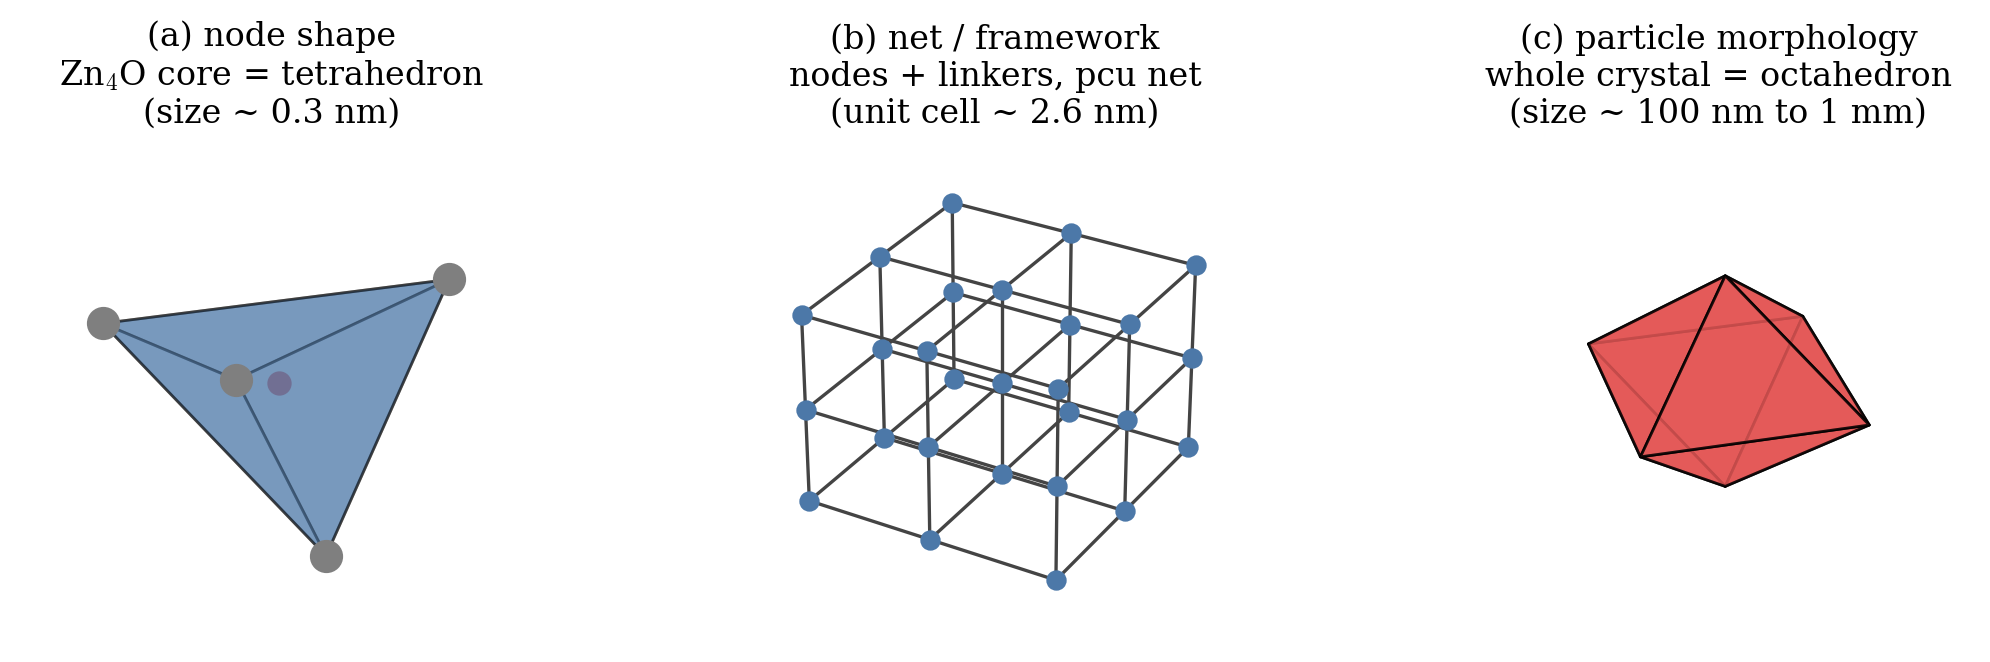
\includegraphics[width=\linewidth]{levels.png}
\caption{Three meanings of ``shape''. (a) The shape of one building unit, such as the tetrahedral Zn$_4$O core of MOF-5 (about 0.3\,nm). (b) The shape of the network formed by nodes and linkers, inside one unit cell (about 2.6\,nm for MOF-5). (c) The outer shape of the whole crystal particle, called its \emph{morphology} or \emph{habit} (100\,nm to millimetres). The panel's question is about (c).}
\label{fig:levels}
\end{figure}

\begin{keyidea}
The panel is asking about level (c), the morphology of the whole crystal. The input is level (b), the unit cell. A single crystal of one MOF contains billions of identical unit cells. The same unit cell can be stacked into an octahedron, a cube, a plate or a rod. Which one forms depends on how fast each crystal face grows.
\end{keyidea}

Our task therefore has three parts:
\begin{enumerate}
\item From the unit cell, find which crystal faces can exist and how fast each should grow. This is \emph{geometry and symmetry}, Parts II and III.
\item Show mathematically that changing the relative growth rates moves the shape continuously between octahedron, cuboctahedron, cube, plate and rod, and measure the shapes with numbers. This is \emph{mathematics}, Part IV.
\item Add the chemistry and graph structure that decide the growth rates in a real MOF. This is Parts V and VI.
\end{enumerate}

\section{What a MOF is}

A \textbf{metal--organic framework (MOF)} is a crystal built from two kinds of pieces:
\begin{itemize}
\item \textbf{Nodes}, also called secondary building units (SBUs): small clusters of metal atoms and oxygen. Examples are the Zn$_4$O cluster in MOF-5, the Cu$_2$ ``paddlewheel'' in HKUST-1 and the Zr$_6$O$_4$(OH)$_4$ cluster in UiO-66.
\item \textbf{Linkers}: organic molecules that bridge nodes. Examples are BDC (benzene-1,4-dicarboxylate, a straight two-ended linker) and BTC (benzene-1,3,5-tricarboxylate, a three-ended linker).
\end{itemize}
Nodes and linkers repeat in three dimensions and leave large empty pores, which is why MOFs adsorb gases. The pattern of connections, ignoring the atoms, is called the \textbf{net} or \textbf{topology}. It has a three-letter name: MOF-5 is \textbf{pcu} (primitive cubic), HKUST-1 is \textbf{tbo}, UiO-66 is \textbf{fcu}, and ZIF-8 is \textbf{sod} (sodalite).

\autoref{fig:mofs} shows the four MOFs we use as test cases. Their crystal files (CIFs) are already in our project folder.

\begin{figure}[H]\centering
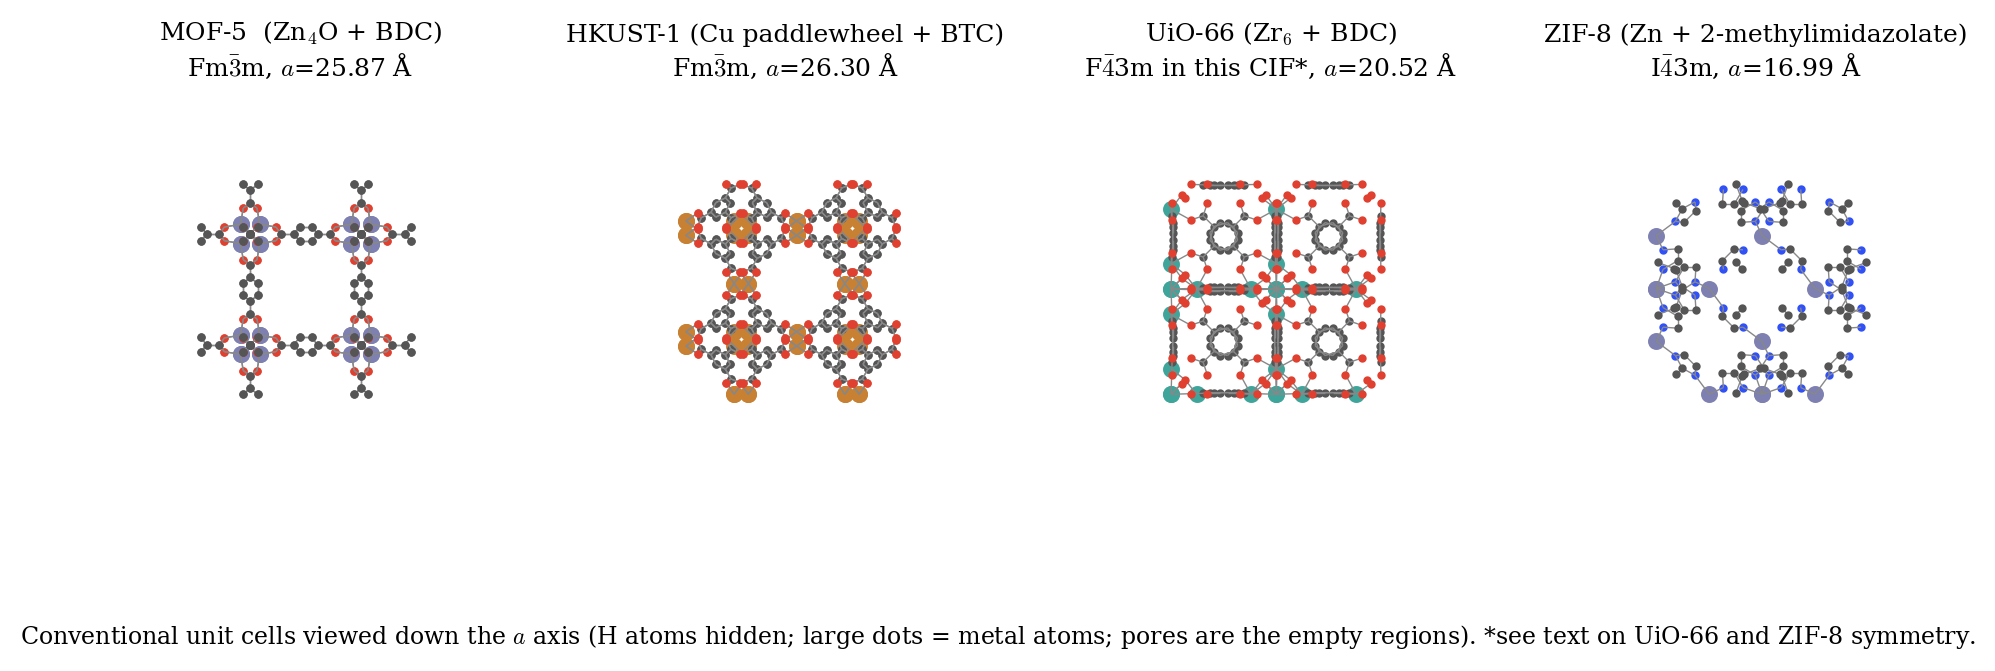
\includegraphics[width=\linewidth]{mofs.png}
\caption{Conventional unit cells of our four test MOFs, drawn from our CIF files and viewed down one axis. Large dots are metal atoms. The empty regions are pores. Space groups and cell lengths were determined by us with the program spglib (\autoref{sec:ourmofs}).}
\label{fig:mofs}
\end{figure}

\begin{table}[H]\centering\small
\begin{tabular}{lllll}
\toprule
MOF & Node & Linker & Net & Lattice type \\
\midrule
MOF-5 & Zn$_4$O (tetrahedral core) & BDC & pcu & F-centred cubic \\
HKUST-1 (Cu-BTC) & Cu$_2$ paddlewheel (square) & BTC (triangle) & tbo & F-centred cubic \\
UiO-66 & Zr$_6$ cluster (octahedral) & BDC & fcu & F-centred cubic \\
ZIF-8 & single Zn (tetrahedral) & 2-methylimidazolate & sod & I-centred cubic \\
\bottomrule
\end{tabular}
\caption{The four test MOFs. ``F-centred'' and ``I-centred'' are explained in \autoref{sec:symmetry}.}
\end{table}

%=====================================================================
\part{Crystal basics}
%=====================================================================
\section{Lattices and unit cells}\label{sec:lattice}

A crystal is a pattern that repeats in space. To describe it we need two things.

\begin{definition}[Lattice]
A \textbf{lattice} is the set of all points $\vect{r} = u\vect{a} + v\vect{b} + w\vect{c}$ with integers $u,v,w$. The three vectors $\vect{a},\vect{b},\vect{c}$ are the \textbf{lattice vectors}.
\end{definition}

\begin{definition}[Unit cell and basis]
The parallelepiped spanned by $\vect{a},\vect{b},\vect{c}$ is a \textbf{unit cell}. The atoms inside one unit cell are the \textbf{basis}. Copying the basis to every lattice point rebuilds the whole crystal.
\end{definition}

A unit cell is described by six numbers: the lengths $a,b,c$ and the angles $\alpha,\beta,\gamma$. This is exactly what the panel calls ``unit cell dimensions''. A cubic cell has $a=b=c$ and all angles $90^\circ$.

\paragraph{Fractional coordinates.} An atom's position is written as $\vect{x}=(x,y,z)$, meaning $\vect{r}=x\vect{a}+y\vect{b}+z\vect{c}$, with $0\le x,y,z<1$ inside the cell. CIF files store positions this way.

\paragraph{Primitive and conventional cells.} The same lattice can be described by different unit cells (\autoref{fig:lattice}). A \textbf{primitive} cell contains exactly one lattice point. A \textbf{conventional} cell may contain more than one, but its edges line up with the symmetry, which makes it much easier to read.

\begin{figure}[H]\centering
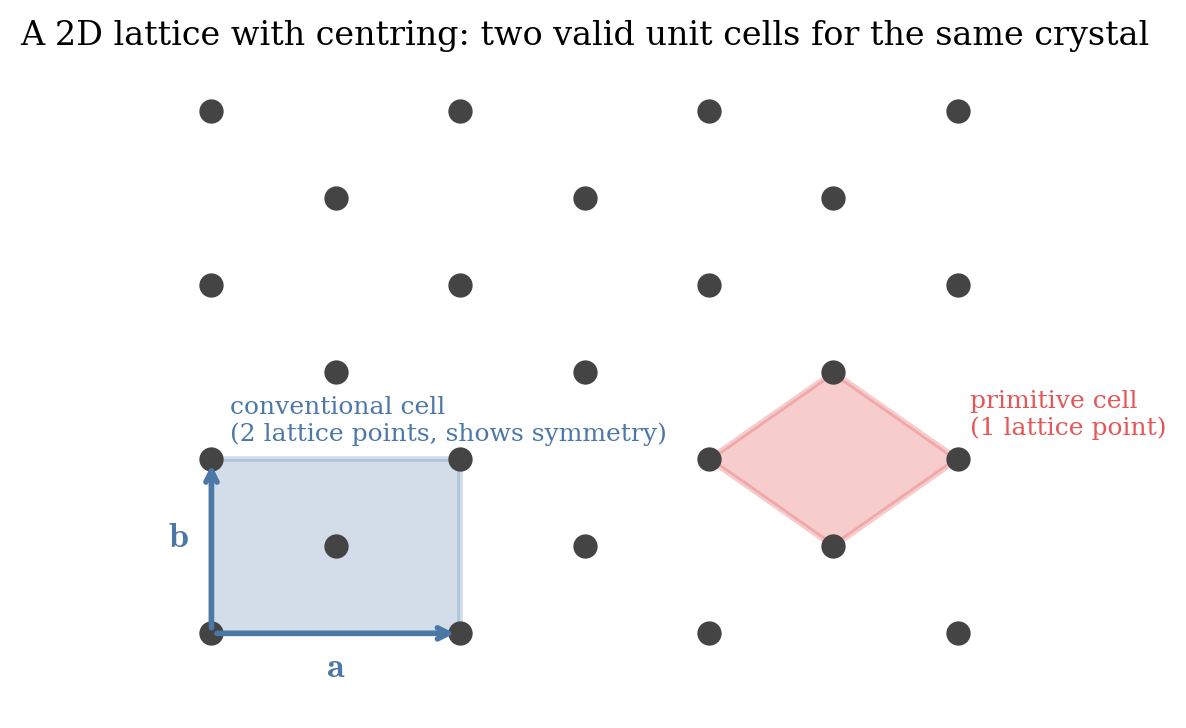
\includegraphics[width=.72\linewidth]{lattice2d.png}
\caption{The same 2D crystal described by two unit cells. The blue conventional cell shows the rectangular symmetry and has an extra lattice point in its centre (``centring''). The red primitive cell has one lattice point but hides the symmetry.}
\label{fig:lattice}
\end{figure}

\begin{careful}
Our HKUST-1 and UiO-66 CIF files store the \emph{primitive} cell, with $a=18.59$\,\AA\ and angles of $60^\circ$ for HKUST-1, and $a=14.51$\,\AA\ and $60^\circ$ for UiO-66. They look non-cubic, but both are cubic. The conventional cubic cells have $a=26.30$\,\AA\ and $a=20.52$\,\AA, since $a_{\text{conv}}=\sqrt2\,a_{\text{prim}}$ for an F-centred lattice. Always convert to the conventional cell before computing faces, or the Miller indices will be meaningless.
\end{careful}

\paragraph{The metric tensor.} Put the lattice vectors as rows of a $3\times3$ matrix $L$. The \textbf{metric tensor} $G=LL^{\mathsf T}$ holds all the dot products $\vect{a}\cdot\vect{a},\vect{a}\cdot\vect{b},\dots$. The length of any lattice vector with fractional components $\vect{u}$ is $|\vect{r}|=\sqrt{\vect{u}^{\mathsf T}G\,\vect{u}}$. For a cubic cell, $G=a^2 I$.

\section{Crystal planes, Miller indices and $d$-spacing}\label{sec:planes}

A crystal \emph{face} is a flat surface parallel to a family of lattice planes. To talk about faces we need a way to name planes.

\begin{definition}[Miller indices]
Take a plane that cuts the three axes at $\vect{a}/h$, $\vect{b}/k$, $\vect{c}/l$. Its \textbf{Miller indices} are the integers $(hkl)$, reduced to have no common factor. A zero means the plane is parallel to that axis. A negative index is written with a bar, for example $(1\bar{1}0)$. The set of all planes related by symmetry is written with curly brackets: $\{100\}$ means all six cube faces $(100),(\bar100),(010),(0\bar10),(001),(00\bar1)$.
\end{definition}

\begin{figure}[H]\centering
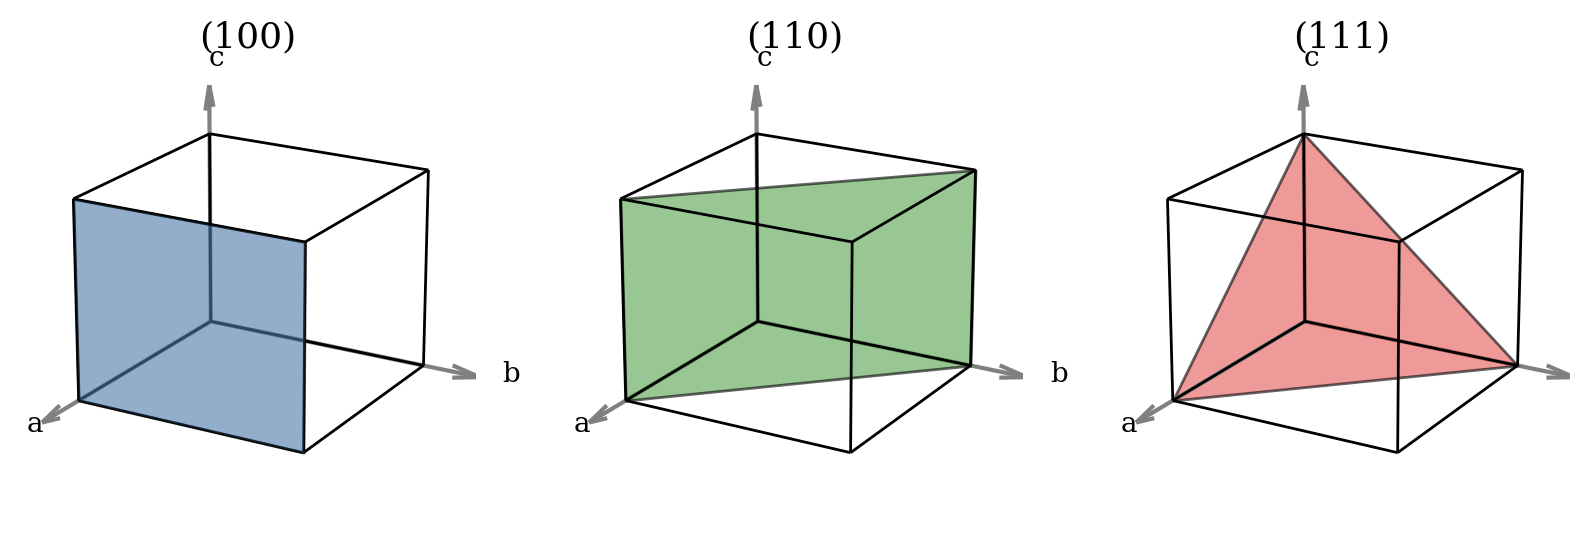
\includegraphics[width=.85\linewidth]{miller.png}
\caption{The three most important plane families in a cubic crystal. $(100)$ cuts only the $a$ axis and is a cube face. $(110)$ cuts $a$ and $b$ equally. $(111)$ cuts all three axes equally and is an octahedron face.}
\label{fig:miller}
\end{figure}

\begin{keyidea}
A cube is bounded by the six $\{100\}$ planes. An octahedron is bounded by the eight $\{111\}$ planes. A rhombic dodecahedron is bounded by the twelve $\{110\}$ planes. So naming the faces that survive \emph{is} naming the shape.
\end{keyidea}

\paragraph{Interplanar spacing $d_{hkl}$.} A family $(hkl)$ is a stack of equally spaced parallel planes. Their spacing is $d_{hkl}$ (\autoref{fig:dspacing}). The higher the indices, the closer together the planes.

\begin{figure}[H]\centering
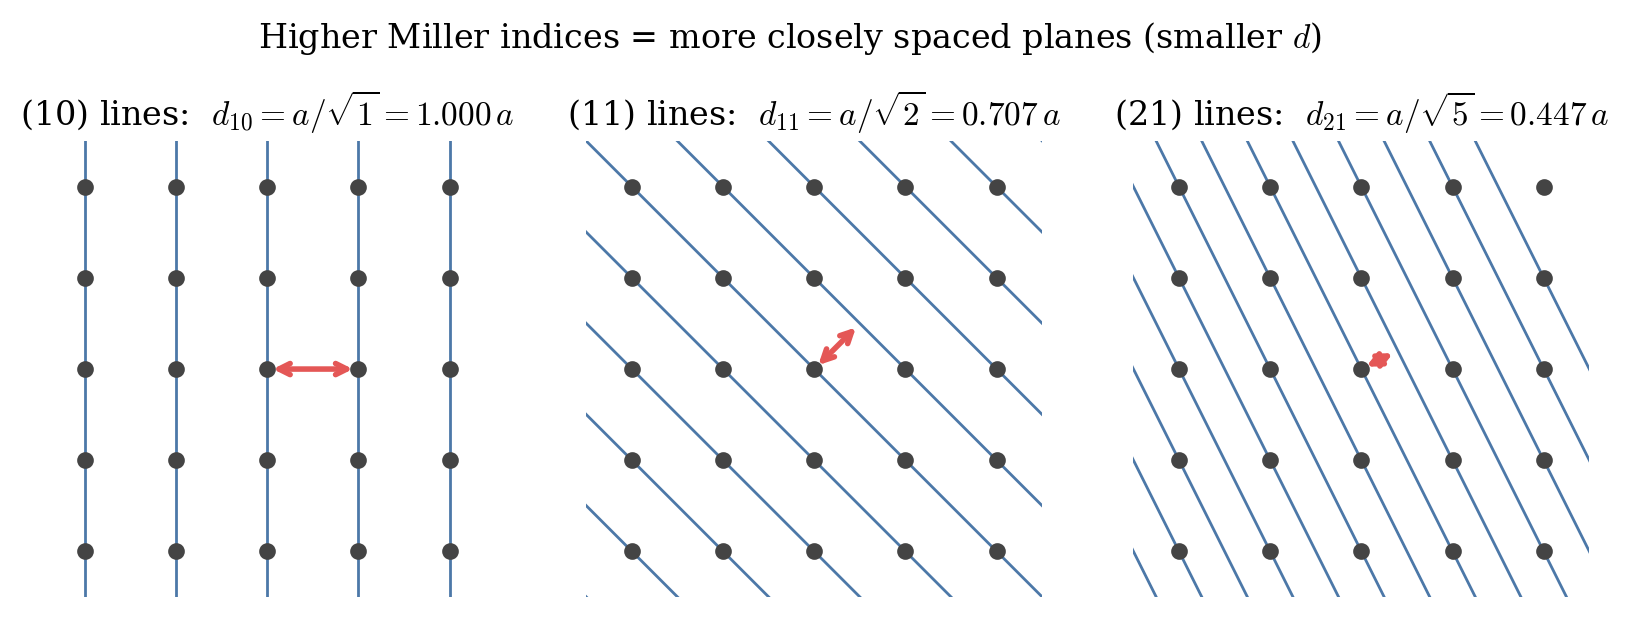
\includegraphics[width=\linewidth]{dspacing.png}
\caption{Plane families in a 2D square lattice. The spacing (red arrow) shrinks as the indices grow: $d_{10}=a$, $d_{11}=a/\sqrt2$, $d_{21}=a/\sqrt5$.}
\label{fig:dspacing}
\end{figure}

\paragraph{The reciprocal lattice.} Define $B=(L^{-1})^{\mathsf T}$. Its rows $\vect{a}^*,\vect{b}^*,\vect{c}^*$ are the \textbf{reciprocal lattice vectors}, with $\vect{a}\cdot\vect{a}^*=1$, $\vect{a}\cdot\vect{b}^*=0$ and so on. The vector
\begin{equation}
\vect{g}_{hkl}=h\vect{a}^*+k\vect{b}^*+l\vect{c}^*
\end{equation}
is perpendicular to the planes $(hkl)$, and its length is $1/d_{hkl}$:
\begin{equation}\label{eq:d}
\frac{1}{d_{hkl}^2}=|\vect{g}_{hkl}|^2=\vect{h}^{\mathsf T}G^{-1}\vect{h},\qquad \vect{h}=(h,k,l)^{\mathsf T}.
\end{equation}
For a cubic cell this becomes the formula to remember:
\begin{equation}\label{eq:dcubic}
d_{hkl}=\frac{a}{\sqrt{h^2+k^2+l^2}}.
\end{equation}

\begin{example}
For MOF-5, $a=25.866$\,\AA. Then $d_{111}=25.866/\sqrt3=14.93$\,\AA, $d_{200}=12.93$\,\AA\ and $d_{220}=9.15$\,\AA. \autoref{tab:d} lists the values we use.
\end{example}

\begin{table}[H]\centering\small
\begin{tabular}{lcl}
\toprule
MOF & $a$ (\AA) & Largest allowed spacings $d$ (\AA) \\
\midrule
MOF-5 & 25.866 & $d_{111}=14.93$, $d_{200}=12.93$, $d_{220}=9.15$, $d_{311}=7.80$\\
HKUST-1 & 26.297 & $d_{111}=15.18$, $d_{200}=13.15$, $d_{220}=9.30$, $d_{311}=7.93$\\
UiO-66 & 20.518 & $d_{111}=11.85$, $d_{200}=10.26$, $d_{220}=7.25$, $d_{311}=6.19$\\
ZIF-8 & 16.991 & $d_{110}=12.01$, $d_{200}=8.50$, $d_{211}=6.94$, $d_{310}=5.37$\\
\bottomrule
\end{tabular}
\caption{Interplanar spacings computed from our CIFs with \eqref{eq:dcubic}. Only the \emph{allowed} families are listed: $(100)$ and $(110)$ are missing for the F-centred MOFs, and $(100)$ and $(111)$ for ZIF-8. The next section explains why.}
\label{tab:d}
\end{table}

\section{Symmetry and which faces are allowed}\label{sec:symmetry}

\subsection{Symmetry operations and space groups}
A \textbf{symmetry operation} is a movement that maps the crystal onto itself. In fractional coordinates every symmetry operation has the form
\begin{equation}
\vect{x}\;\mapsto\;R\,\vect{x}+\vect{t},
\end{equation}
where $R$ is a $3\times3$ integer matrix (a rotation, reflection or inversion) and $\vect{t}$ is a translation. Three kinds of translations matter:
\begin{itemize}
\item \textbf{Centring}: $R=I$ and $\vect{t}$ is a fraction of a cell. F-centring adds $(0,\tfrac12,\tfrac12)$, $(\tfrac12,0,\tfrac12)$ and $(\tfrac12,\tfrac12,0)$, which are atoms at the face centres. I-centring adds $(\tfrac12,\tfrac12,\tfrac12)$, an atom at the body centre.
\item \textbf{Screw axes}: a rotation combined with a partial translation along the axis.
\item \textbf{Glide planes}: a reflection combined with a partial translation within the plane.
\end{itemize}
The full set of symmetry operations of a crystal is its \textbf{space group}. There are exactly 230 of them, each with a symbol such as Fm$\bar3$m (number 225). The symbol's first letter gives the centring: P (primitive), I (body-centred) or F (face-centred).

\subsection{Systematic absences: why some faces cannot exist}
Centring, screw axes and glide planes create extra, identical planes between the planes of a family. \autoref{fig:abs} shows this for F-centring. Waves scattered from the $(100)$ planes and from the identical planes halfway between them cancel exactly. Physically, the true repeat distance perpendicular to $(100)$ is then $a/2$, not $a$. This is called a \textbf{systematic absence}. The rule can be proved in two lines.

\begin{proposition}[Systematic absence rule]\label{prop:abs}
Let $F(\vect{h})=\sum_j f_j\,e^{2\pi i\,\vect{h}\cdot\vect{x}_j}$ be the structure factor of a reflection $\vect{h}=(h,k,l)$, summed over all atoms $j$ in the cell. If the space group contains an operation $(R,\vect{t})$ with $\vect{h}R=\vect{h}$ and $\vect{h}\cdot\vect{t}\notin\mathbb{Z}$, then $F(\vect{h})=0$.
\end{proposition}
\begin{proof}
The operation maps the set of atoms onto itself, so we may sum over the images $R\vect{x}_j+\vect{t}$ instead of $\vect{x}_j$:
$F(\vect{h})=\sum_j f_j e^{2\pi i\,\vect{h}\cdot(R\vect{x}_j+\vect{t})}=e^{2\pi i\,\vect{h}\cdot\vect{t}}\sum_j f_j e^{2\pi i\,(\vect{h}R)\cdot\vect{x}_j}=e^{2\pi i\,\vect{h}\cdot\vect{t}}F(\vect{h}R)$.
If $\vect{h}R=\vect{h}$ this reads $F(\vect{h})(1-e^{2\pi i\,\vect{h}\cdot\vect{t}})=0$. The bracket is non-zero when $\vect{h}\cdot\vect{t}$ is not an integer, so $F(\vect{h})=0$.
\end{proof}

Applying the rule to pure centring ($R=I$) gives the two rules we need:
\begin{itemize}
\item \textbf{F-centred}: $(hkl)$ is allowed only if $h,k,l$ are \emph{all even or all odd}. So $(100)$ and $(110)$ are absent, while $(111)$, $(200)$ and $(220)$ are allowed.
\item \textbf{I-centred}: $(hkl)$ is allowed only if $h+k+l$ is \emph{even}. So $(100)$ and $(111)$ are absent, while $(110)$, $(200)$ and $(211)$ are allowed.
\end{itemize}

\begin{figure}[H]\centering
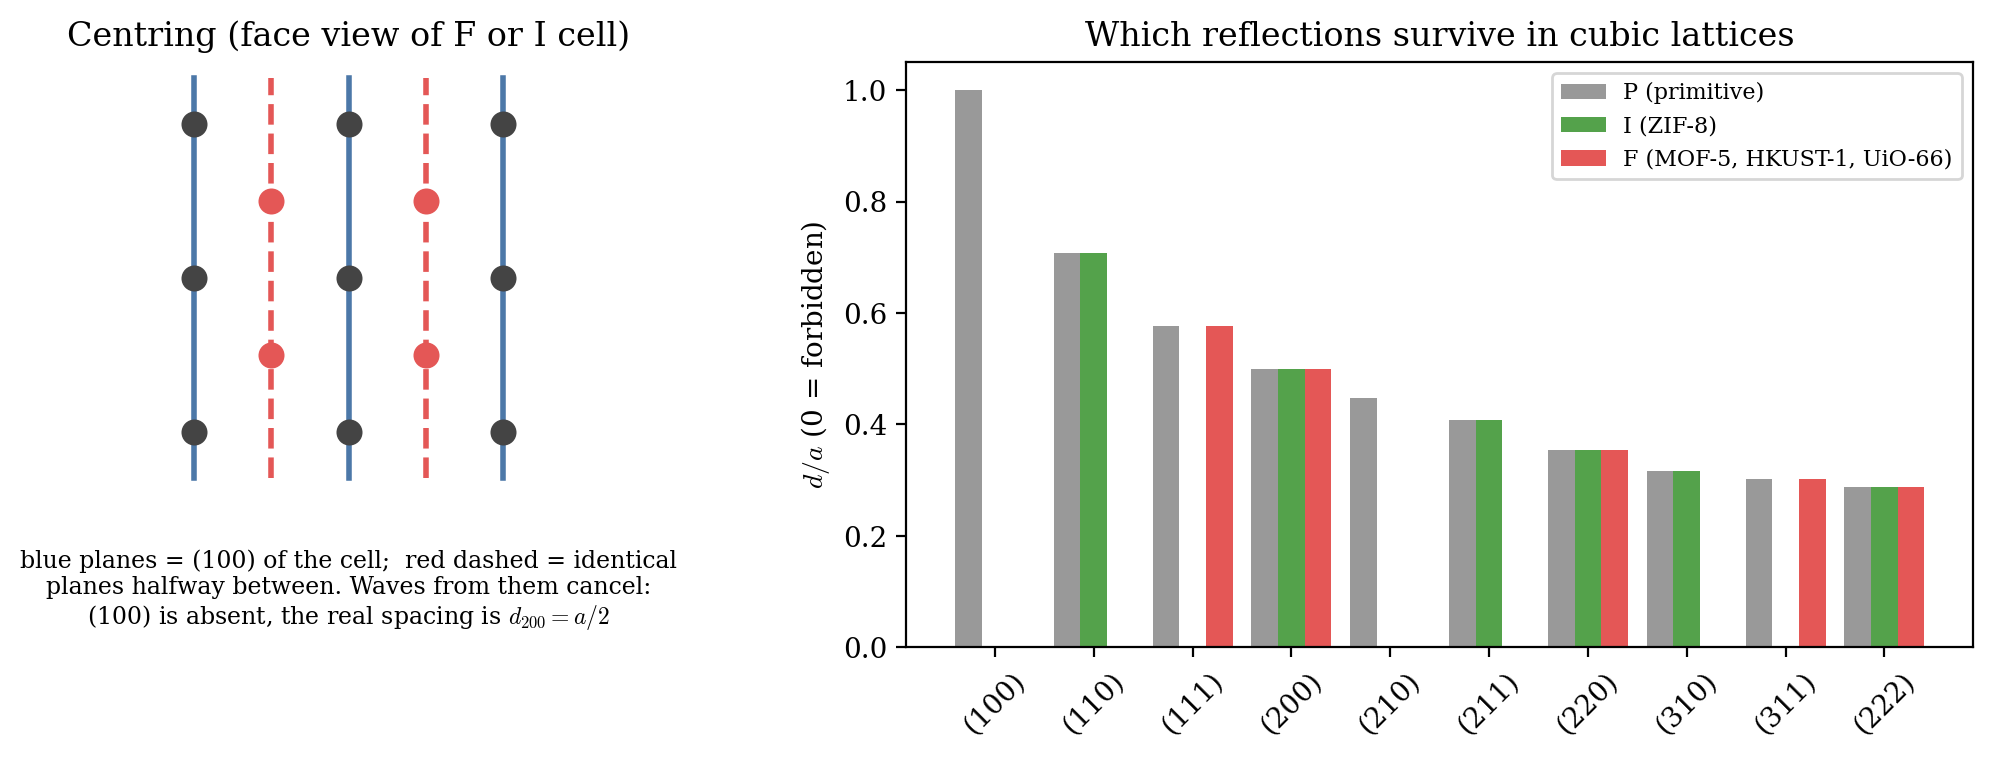
\includegraphics[width=\linewidth]{absences.png}
\caption{Left: centring puts identical planes (red dashed) halfway between the $(100)$ planes (blue), so the true spacing is $a/2$. Right: the spacing $d/a$ of each family in primitive (P), body-centred (I, ZIF-8) and face-centred (F, MOF-5, HKUST-1, UiO-66) cubic lattices. Zero means forbidden.}
\label{fig:abs}
\end{figure}

\begin{definition}[Effective spacing]
For a direction $(hkl)$, let $n$ be the smallest positive integer for which $(nh\,nk\,nl)$ is allowed. The \textbf{effective spacing} is $d_{\text{eff}}=d_{hkl}/n$. For an F-centred cubic crystal the cube-face direction has $d_{\text{eff}}=d_{200}=a/2$, not $a$.
\end{definition}

This correction was introduced by Donnay and Harker (1937). It matters greatly for MOFs: without it, a program would predict cube faces for MOF-5 based on $d_{100}=a$, which is wrong.

\subsection{The symmetry of our four MOFs}\label{sec:ourmofs}
All four of our CIFs are stored in space group P1, meaning no symmetry is written in the file. We detected the true space groups with the program spglib at tolerances from 0.001 to 0.05\,\AA:
\begin{itemize}
\item MOF-5: Fm$\bar3$m (225), $a=25.866$\,\AA.
\item HKUST-1: Fm$\bar3$m (225), conventional $a=26.297$\,\AA.
\item UiO-66: F$\bar4$3m (216), conventional $a=20.518$\,\AA. The literature usually gives Fm$\bar3$m for UiO-66. Our file orders the $\mu_3$-O and $\mu_3$-OH groups in the cluster, which removes the inversion centre. The centring is still F, so the allowed faces are the same.
\item ZIF-8: with hydrogen atoms included, spglib finds only P1, because the hydrogen positions in our file break the symmetry. Without hydrogens it finds I$\bar4$3m (217), the accepted space group.
\end{itemize}

\begin{careful}
Always check the symmetry, both with and without hydrogens and at more than one tolerance. A wrong space group gives wrong allowed faces, and therefore a wrong shape.
\end{careful}

%=====================================================================
\part{How a crystal gets its shape}
%=====================================================================
\section{Growth: the slowest faces win}

A crystal grows by adding molecules or building blocks to its surface. Each face moves outward at its own speed, called the \textbf{normal growth rate} $R_{hkl}$. \autoref{fig:growth} shows a simple 2D simulation: a crystal starts with eight faces, four slow and four fast.

\begin{figure}[H]\centering
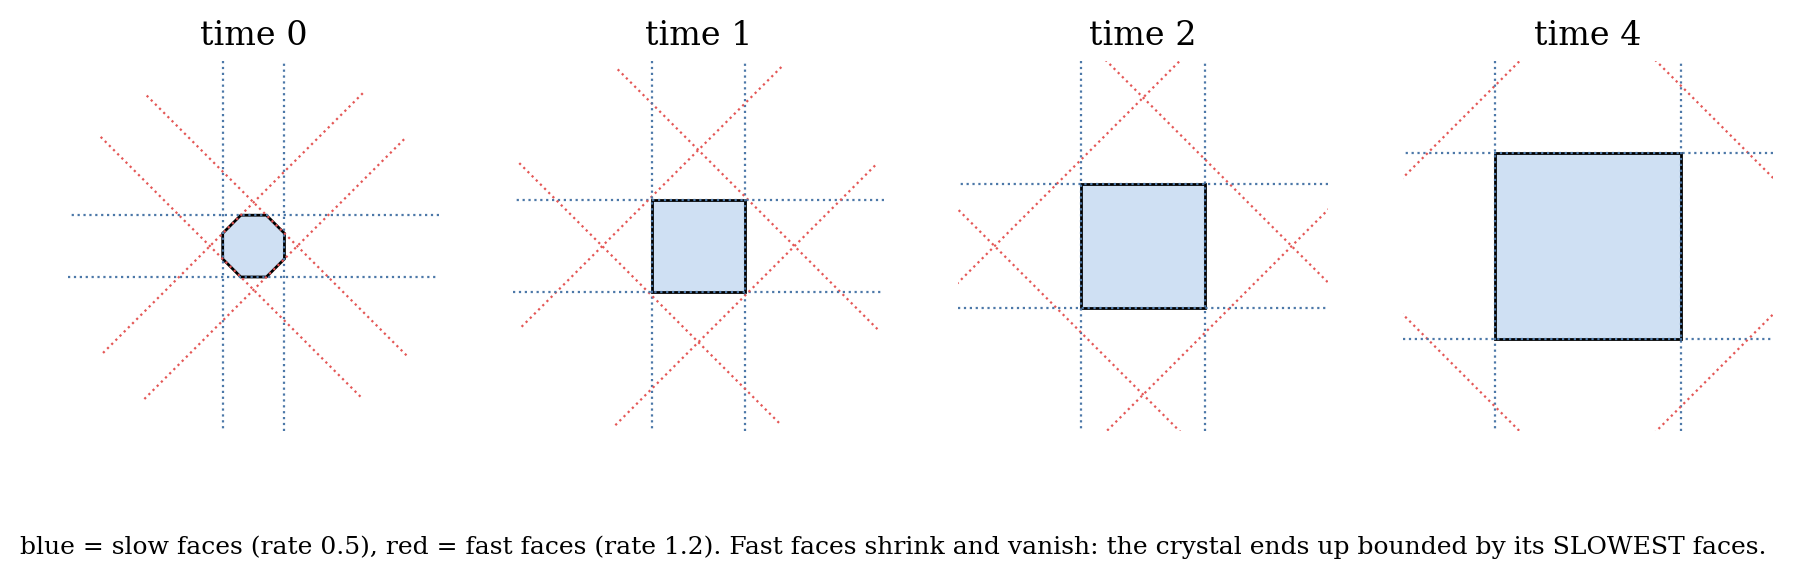
\includegraphics[width=\linewidth]{growth.png}
\caption{2D growth with four slow faces (blue, rate 0.5) and four fast faces (red, rate 1.2). The fast faces shrink and disappear. At late times the crystal is a square bounded only by the slow faces.}
\label{fig:growth}
\end{figure}

\begin{keyidea}
Fast-growing faces grow themselves out of existence. The final crystal is bounded by its \textbf{slowest-growing} faces. The distance of each face from the crystal's centre is proportional to its growth rate:
\begin{equation}\label{eq:central}
h_{hkl}\;\propto\;R_{hkl}.
\end{equation}
So predicting a crystal's shape means predicting the relative growth rates of its faces. Everything in Part III is a way of estimating $R_{hkl}$.
\end{keyidea}

Mathematically, the shape at late times is the region
\begin{equation}\label{eq:polytope}
P=\{\vect{x}\in\mathbb{R}^3:\ \hat{\vect{n}}_{hkl}\cdot\vect{x}\le R_{hkl}\ \text{for every face } (hkl)\},
\end{equation}
where $\hat{\vect{n}}_{hkl}$ is the unit vector perpendicular to the face, the direction of $\vect{g}_{hkl}$. This is an intersection of half-spaces. It is always a convex polyhedron, and we study it in Part IV.

\section{BFDH: shape from the unit cell alone}\label{sec:bfdh}

The oldest rule for estimating $R_{hkl}$ uses only the lattice. It is named after Bravais, Friedel, Donnay and Harker (BFDH).

\begin{keyidea}[title=BFDH law]
Planes that are far apart ($d$ large) are densely packed and strongly bonded within themselves, so they grow slowly. The growth rate is taken as
\begin{equation}\label{eq:bfdh}
R_{hkl}\;\propto\;\frac{1}{d_{\text{eff}}(hkl)}.
\end{equation}
The faces with the \emph{largest} effective spacings dominate the shape.
\end{keyidea}

BFDH needs only the unit cell and the space group, which is exactly the input the panel specified. It is therefore the first answer to their question. \autoref{fig:bfdh} shows the BFDH shapes for our two lattice types, computed by us with \eqref{eq:polytope} and \eqref{eq:bfdh}.

\begin{figure}[H]\centering
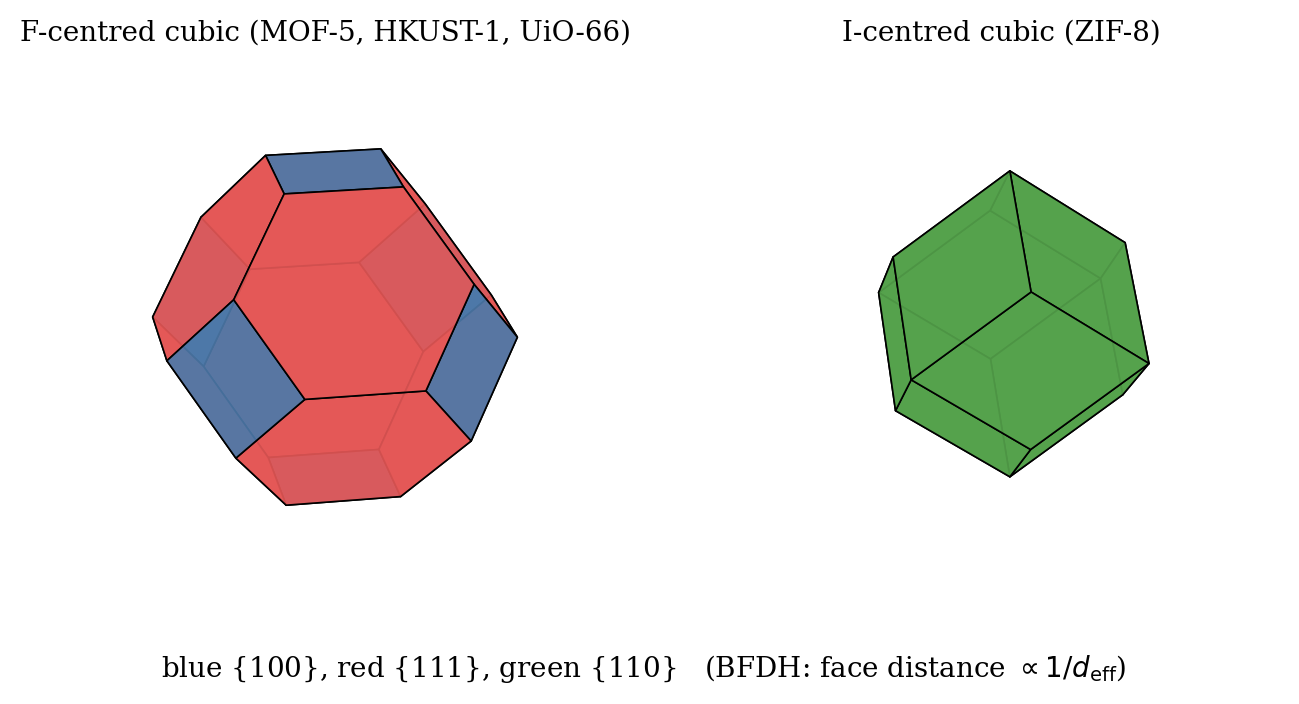
\includegraphics[width=.85\linewidth]{bfdh_FI.png}
\caption{BFDH morphologies computed from the unit cell. Left: F-centred cubic gives an octahedron ($\{111\}$, red) truncated by small cube faces ($\{100\}$, blue), with 8+6 faces. Right: I-centred cubic gives a rhombic dodecahedron with 12 $\{110\}$ faces (green).}
\label{fig:bfdh}
\end{figure}

\begin{example}[F-centred, MOF-5, HKUST-1 and UiO-66]
The allowed families with the largest $d$ are $\{111\}$ with $d=a/\sqrt3=0.577a$ and $\{200\}$ with $d=a/2$. By \eqref{eq:bfdh} the face distances are $\sqrt3=1.732$ and $2$ (in units of $1/a$). Their ratio is $1.732/2=0.866$. Part IV shows that this ratio gives a truncated octahedron. The $\{220\}$ planes lie further out and do not appear.
\end{example}

\begin{example}[I-centred, ZIF-8]
The largest allowed spacing is $\{110\}$ with $d=a/\sqrt2$, which gives a rhombic dodecahedron. The $\{200\}$ planes ($d=a/2$) only touch its corners.
\end{example}

\begin{forus}
These BFDH shapes can be compared with what labs see. ZIF-8 is widely reported to grow as rhombic dodecahedra, which matches BFDH. UiO-67 (the same fcu net and F-centring as UiO-66) grows as cuboctahedra and then octahedra (Chen et al., \autoref{sec:chen}), close to the $\{111\}$-dominated BFDH shape. HKUST-1 is commonly octahedral. MOF-5 is usually reported as cubes, which BFDH does \emph{not} predict. \autoref{sec:attach} shows that a simple graph rule fixes this. We still have to collect specific references for these experimental shapes in Phase~0 of the plan.
\end{forus}

\section{Wulff construction: shape from surface energy}\label{sec:wulff}

BFDH ignores chemistry. A better estimate of which faces win uses the \textbf{surface energy} $\gamma_{hkl}$: the energy cost per unit area of creating face $(hkl)$. A crystal in equilibrium minimises its total surface energy for a fixed volume, a principle due to Gibbs.

\begin{proposition}[Wulff theorem]\label{prop:wulff}
Let $\gamma(\hat{\vect{n}})>0$ be the surface energy in direction $\hat{\vect{n}}$. Among all bodies of a given volume, the one with the smallest total surface energy $\int\gamma(\hat{\vect{n}})\,dA$ is, up to scaling and translation, the \textbf{Wulff shape}
\begin{equation}\label{eq:wulff}
W=\{\vect{x}:\ \hat{\vect{n}}\cdot\vect{x}\le\gamma(\hat{\vect{n}})\ \text{for all directions } \hat{\vect{n}}\}.
\end{equation}
\end{proposition}
This is a deep theorem, and we cite it rather than prove it (Wulff 1901; rigorous proofs by J.~E.~Taylor; see the review by Miracle-Sol\'e, arXiv:1307.5180). \autoref{fig:wulff} shows the construction.

\begin{figure}[H]\centering
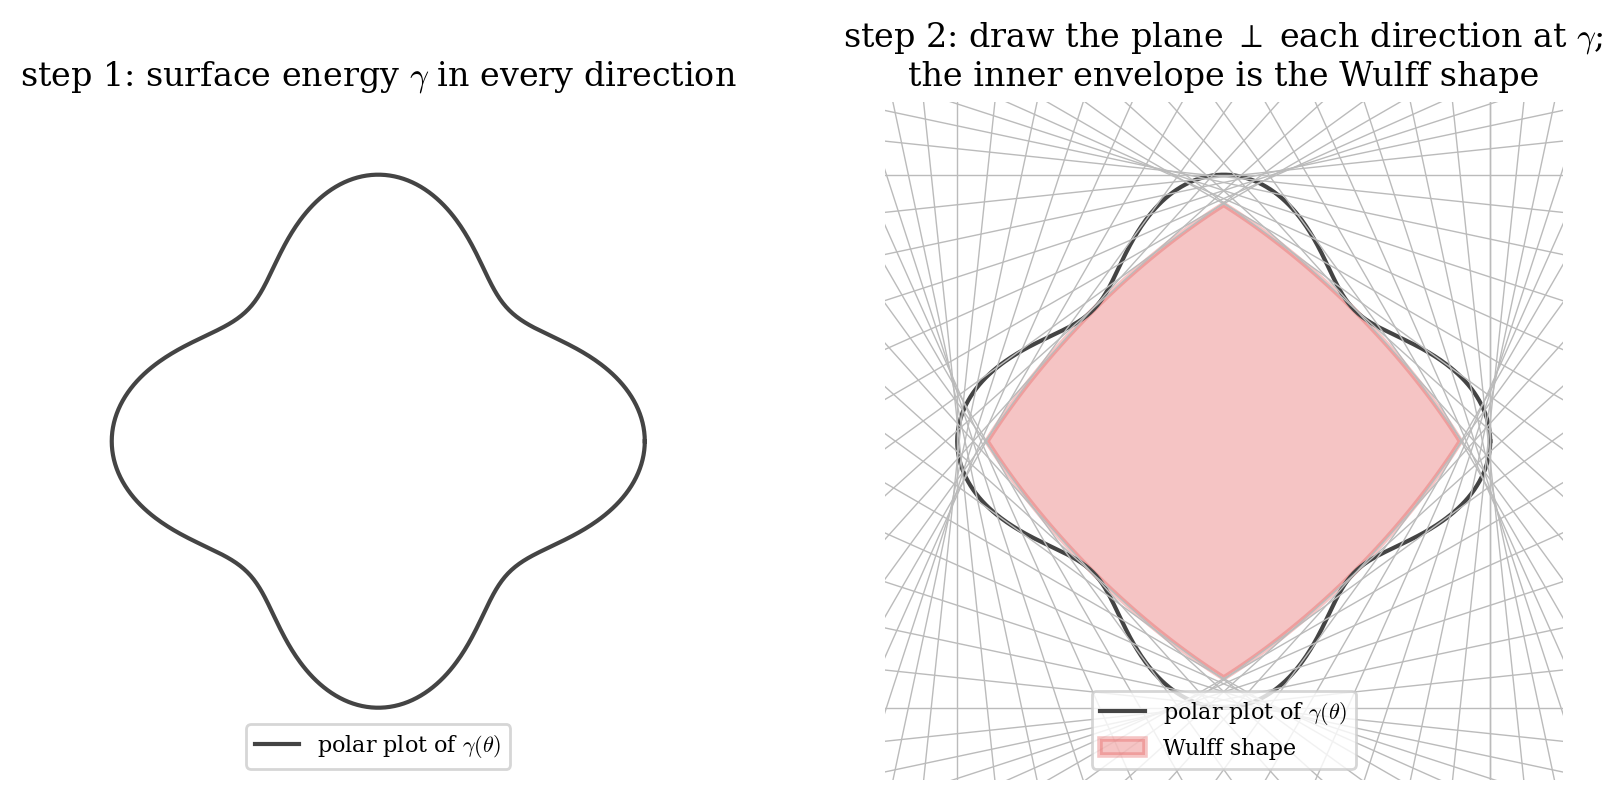
\includegraphics[width=.85\linewidth]{wulff2d.png}
\caption{The Wulff construction in 2D. Left: surface energy plotted in every direction. Right: a line perpendicular to each direction at distance $\gamma$; the region inside all lines (red) is the equilibrium shape. Directions with low $\gamma$ become large faces.}
\label{fig:wulff}
\end{figure}

\begin{keyidea}
Equation \eqref{eq:wulff} has exactly the same form as the growth shape \eqref{eq:polytope}. Only the numbers change: $R_{hkl}$ (growth) or $\gamma_{hkl}$ (equilibrium). The same polytope code serves BFDH, Wulff and every kinetic model. We only swap the input numbers.
\end{keyidea}

\paragraph{Attachment energy.} A third estimate sits between BFDH and Wulff. Cut the crystal into slices of thickness $d_{hkl}$. The lattice energy splits as $E_{\text{latt}}=E_{\text{slice}}+E_{\text{att}}$, where $E_{\text{att}}$ is the energy released when a new slice attaches to the face. Hartman and Bennema (1980) proposed $R_{hkl}\propto|E_{\text{att}}|$: faces that release little energy on attachment grow slowly. This needs a force field to compute the energies, and it is what commercial tools such as Materials Studio Morphology compute.

\section{Hartman--Perdok theory: faces from bond chains}\label{sec:pbc}

Why should some faces grow slowly? Hartman and Perdok (1955) answered with the bonds inside the crystal.

\begin{definition}[Periodic bond chain]
A \textbf{periodic bond chain (PBC)} is an unbroken chain of strong bonds that repeats with a lattice translation $\vect{\tau}$, so it runs through the whole crystal in one direction.
\end{definition}

Consider the slice of thickness $d_{hkl}$ parallel to a face. Count the PBCs that lie entirely within the slice:
\begin{itemize}
\item \textbf{F face} (flat): the slice contains PBCs in two or more independent directions. The face is a strongly bonded layer, and growth needs a whole new layer to nucleate, so it is \emph{slow}. F faces dominate the morphology.
\item \textbf{S face} (stepped): PBCs in exactly one direction. Growth is faster.
\item \textbf{K face} (kinked): no PBC in the slice. Every surface site is a kink, so the face grows fastest and usually disappears.
\end{itemize}

\begin{figure}[H]\centering
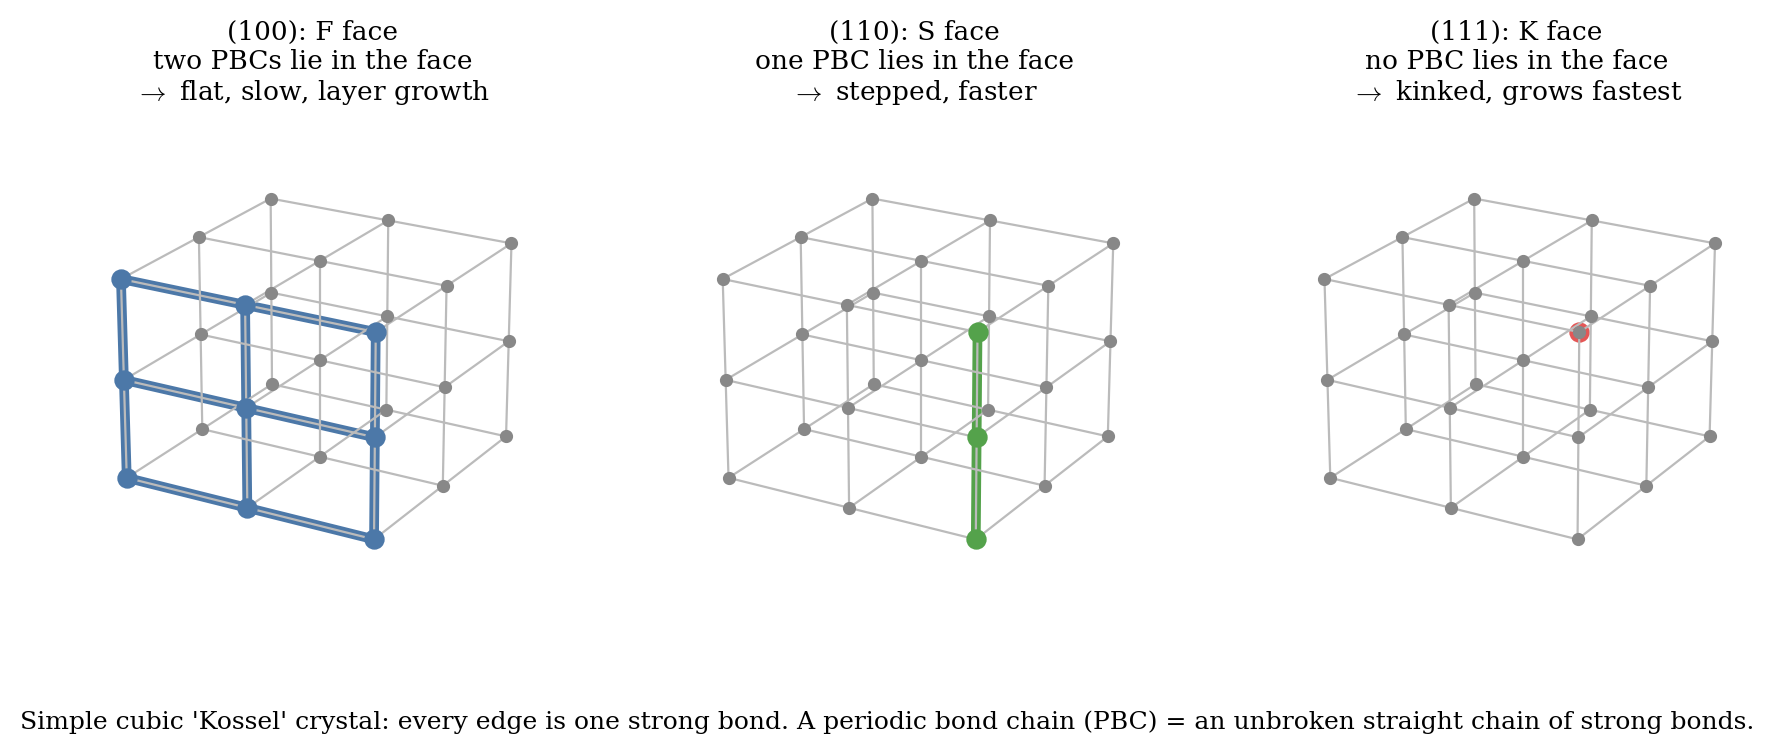
\includegraphics[width=\linewidth]{fsk.png}
\caption{The F/S/K classification in a simple cubic crystal where every edge is a strong bond. (100) contains chains in two directions (F). (110) contains chains in one direction (S). (111) contains none (K). So this crystal grows as a cube.}
\label{fig:fsk}
\end{figure}

\begin{keyidea}
Hartman--Perdok theory turns crystal growth into a question about \emph{how a periodic network of bonds is connected inside a slab}. That is a graph question, and Part V shows that our periodic quotient graph answers it directly.
\end{keyidea}

The theory has been refined since 1955. Hartman's 1982 review states that only F faces containing two or more PBCs grow by a layer mechanism. Grimbergen and co-workers (Acta Cryst.\ A, 1998) restated the theory in terms of \emph{connected nets} and roughening transitions.

%=====================================================================
\part{The mathematics of morphing}
%=====================================================================
\section{Crystal shapes as polytopes, and a continuous morph}\label{sec:morph}

Every shape model in Part III produces a set of the same form:
\begin{equation}
P(\vect{b})=\{\vect{x}\in\mathbb{R}^3:\ A\vect{x}\le\vect{b}\},
\end{equation}
where each row of $A$ is a unit face normal and $\vect{b}$ holds the face distances (growth rates or surface energies).

\begin{proposition}[The shape is a convex polytope with crystal symmetry]\label{prop:convex}
If $\vect{b}>0$ and the normals in $A$ are not all on one side of a plane, then $P(\vect{b})$ is a bounded convex polytope containing the origin. If $\vect{b}$ takes the same value on symmetry-equivalent faces, $P(\vect{b})$ has the point symmetry of the crystal.
\end{proposition}
\begin{proof}[Proof sketch]
An intersection of half-spaces is convex. Because the normals surround the origin, every direction is eventually blocked by some face, so $P$ is bounded. It contains the origin because $\vect{b}>0$. A symmetry $S$ permutes the rows of $A$ and leaves $\vect{b}$ unchanged, so it maps $P$ onto itself.
\end{proof}

\begin{proposition}[Continuity of the morph]\label{prop:cont}
For fixed normals $A$, the map $\vect{b}\mapsto P(\vect{b})$ is continuous in the Hausdorff distance. So are the volume, surface area and gyration tensor of $P(\vect{b})$.
\end{proposition}
This is a standard result in convex geometry (it follows from Hoffman's error bound for linear inequalities). It means that changing the relative growth rates continuously changes the shape continuously. The shape \emph{morphs}, with no jumps.

\subsection{The cube--octahedron family in closed form}
Take a cubic crystal with only $\{100\}$ faces at distance 1 and $\{111\}$ faces at distance $t$. The ratio $t$ is the only parameter. By direct geometry:
\begin{itemize}
\item The $\{111\}$ plane $x+y+z=\sqrt3\,t$ touches the cube corner $(1,1,1)$ when $\sqrt3\,t=3$. So for $t\ge\sqrt3$ the shape is a \textbf{cube}.
\item It passes through the cube edge midpoints $(1,1,0)$ when $\sqrt3\,t=2$. So at $t=2/\sqrt3\approx1.155$ the shape is a \textbf{cuboctahedron}.
\item The octahedron vertex $(\sqrt3\,t,0,0)$ touches the cube face $x=1$ when $t=1/\sqrt3$. So for $t\le1/\sqrt3\approx0.577$ the shape is an \textbf{octahedron}.
\item In between, the shape is a \textbf{truncated cube} ($2/\sqrt3<t<\sqrt3$) or a \textbf{truncated octahedron} ($1/\sqrt3<t<2/\sqrt3$).
\end{itemize}

\begin{figure}[H]\centering
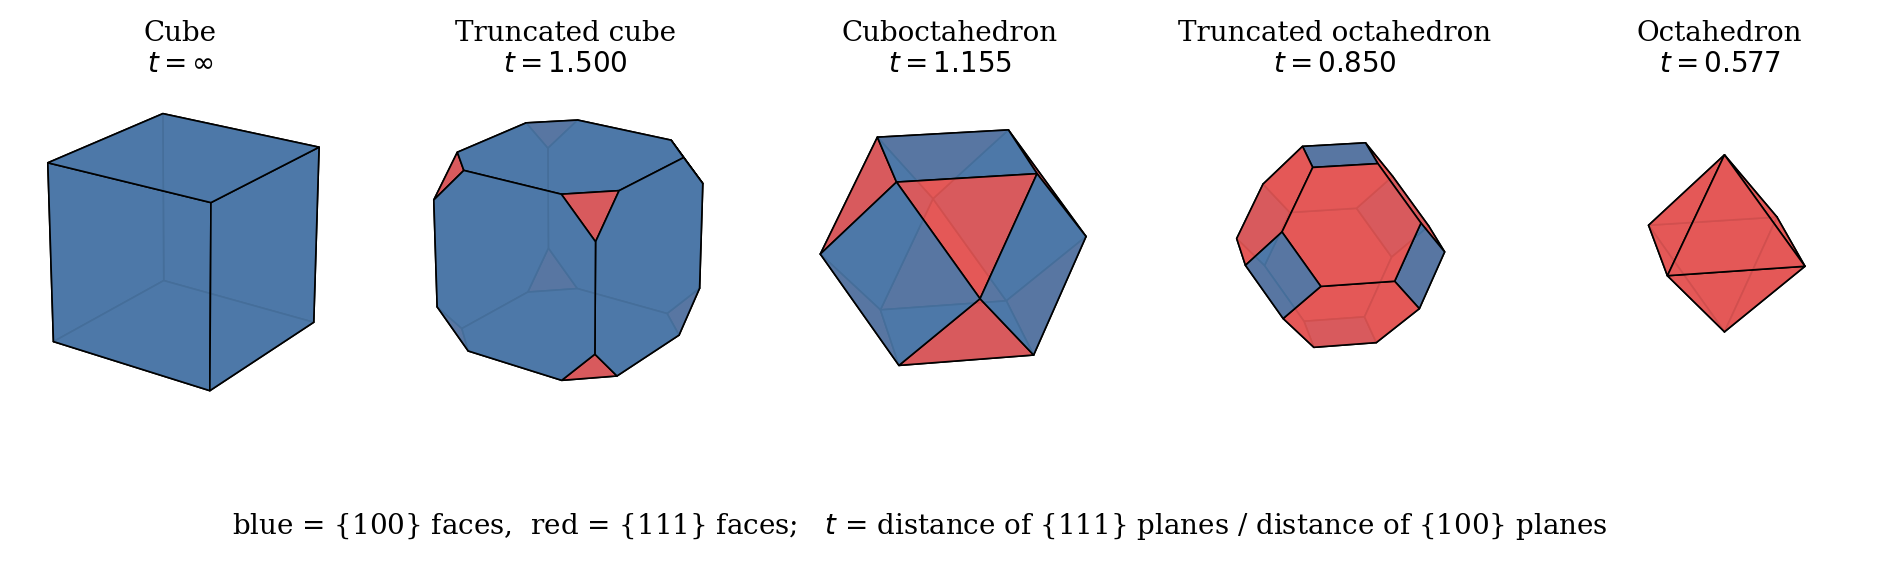
\includegraphics[width=\linewidth]{morph_path.png}
\caption{One continuous morph, computed by us. Lowering the ratio $t$ of $\{111\}$ to $\{100\}$ face distances takes the crystal from cube to octahedron through the truncated cube, cuboctahedron and truncated octahedron. The BFDH value for F-centred MOFs is $t=0.866$, a truncated octahedron.}
\label{fig:morph}
\end{figure}

\begin{keyidea}
This is the mathematical form of the panel's request. One unit cell supports a whole one-parameter family of morphologies, and we can say exactly where each named shape appears. Chemistry then decides the value of $t$, for example by changing solvent or modulator.
\end{keyidea}

\subsection{Plates and rods}
Plates and rods appear when growth along one axis is slower or faster than along the others, for example when a modulator binds to one face family. We model this with a stretch along $z$ by a factor $\lambda$: $\lambda<1$ gives a plate and $\lambda>1$ gives a rod (\autoref{fig:rod}).

\begin{figure}[H]\centering
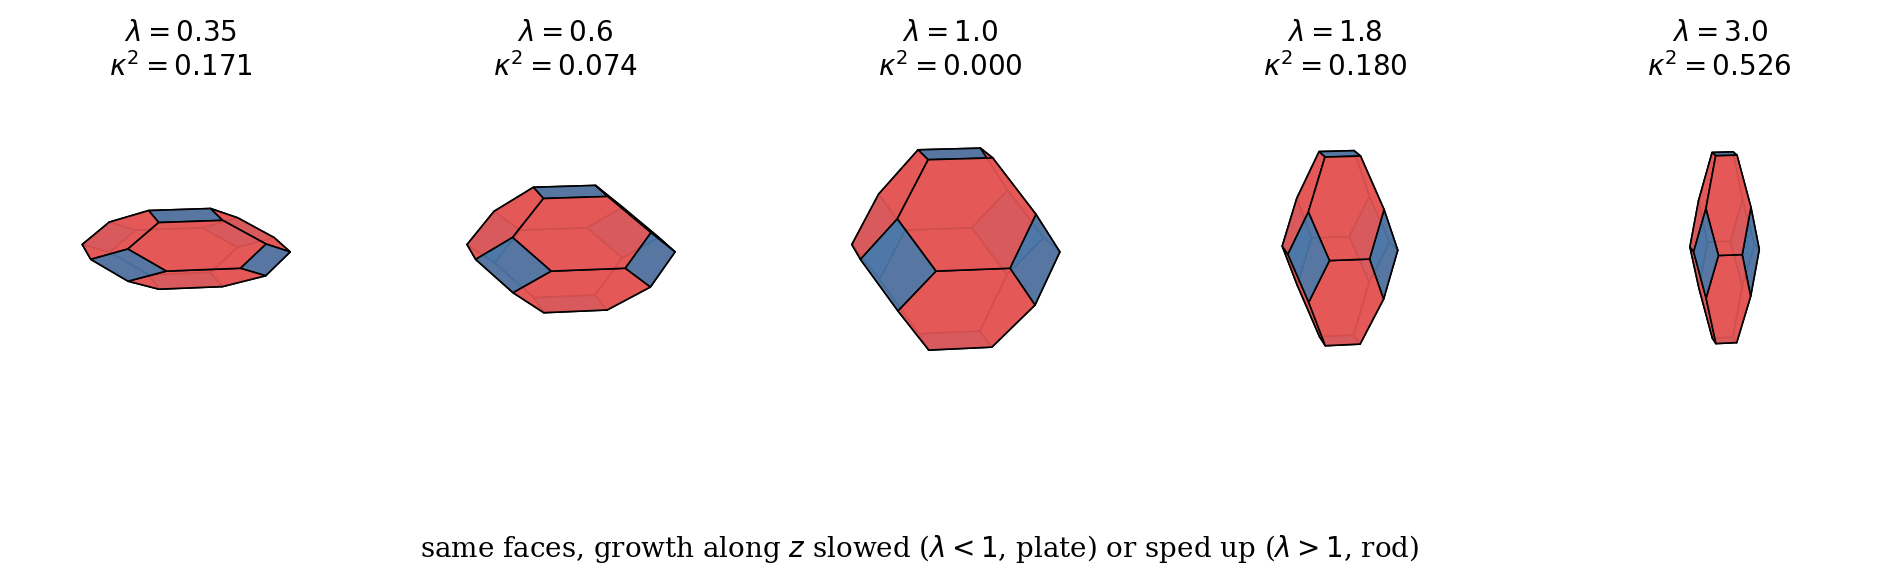
\includegraphics[width=\linewidth]{rod_plate.png}
\caption{The truncated octahedron ($t=0.85$) with growth along $z$ slowed (plates, $\lambda<1$) or sped up (rods, $\lambda>1$). The faces are the same, only their sizes change. $\kappa^2$ measures how far the shape is from isotropic (\autoref{sec:measure}).}
\label{fig:rod}
\end{figure}

\begin{careful}
A uniform stretch is a modelling device. It breaks the cubic symmetry of the growth rates, which in a cubic crystal needs an external cause such as a substrate, a surfactant or a modulator. We must state this clearly when presenting rods and plates.
\end{careful}

\section{Measuring shape with numbers}\label{sec:measure}

To show that shapes are different we need numbers, not pictures.

\paragraph{Gyration tensor.} For a solid body $P$ with centre of mass at the origin,
\begin{equation}
S=\frac{1}{|P|}\int_P \vect{x}\vect{x}^{\mathsf T}\,dV,
\end{equation}
with eigenvalues $\lambda_1\ge\lambda_2\ge\lambda_3$. The \textbf{asphericity} is
\begin{equation}
\kappa^2=\frac32\,\frac{\lambda_1^2+\lambda_2^2+\lambda_3^2}{(\lambda_1+\lambda_2+\lambda_3)^2}-\frac12,
\end{equation}
which is 0 for an isotropic body and 1 for a line. The \textbf{aspect ratio} is $\sqrt{\lambda_1/\lambda_3}$.

\paragraph{Sphericity.} With volume $V$ and surface area $A$,
\begin{equation}
\Psi=\frac{\pi^{1/3}(6V)^{2/3}}{A},
\end{equation}
which equals 1 for a sphere and is smaller for every other shape.

\begin{proposition}[$\kappa^2$ cannot tell cubic shapes apart]\label{prop:k2}
If a body has the symmetry of a cube or a tetrahedron, then $S$ is a multiple of the identity and $\kappa^2=0$.
\end{proposition}
\begin{proof}
Both groups contain the $180^\circ$ rotations about the $x$, $y$ and $z$ axes. Invariance under them forces every off-diagonal entry of $S$ to be zero. Both groups also contain the $120^\circ$ rotation about $(1,1,1)$, which permutes $x\to y\to z$. Invariance under it forces the three diagonal entries to be equal.
\end{proof}

\begin{careful}
So $\kappa^2$ is zero for the cube, octahedron, tetrahedron and sphere alike. In our earlier work we used $\kappa^2$ to separate ``tetrahedral'' from ``spherical'', but for cubic-symmetric shapes that cannot work. We must use sphericity, face counts, or higher-order descriptors such as Steinhardt order parameters of the face normals. $\kappa^2$ is still the right tool for rods and plates.
\end{careful}

\begin{table}[H]\centering\small
\begin{tabular}{lcccc}
\toprule
Shape & Faces & Vertices & Sphericity $\Psi$ & $\kappa^2$\\
\midrule
Cube ($t\ge\sqrt3$) & 6 & 8 & 0.806 & 0\\
Truncated cube ($t=1.5$) & 14 & 24 & 0.828 & 0\\
Cuboctahedron ($t=1.155$) & 14 & 12 & 0.905 & 0\\
Truncated octahedron ($t=0.85$) & 14 & 24 & 0.907 & 0\\
Octahedron ($t\le0.577$) & 8 & 6 & 0.846 & 0\\
BFDH, F-centred ($t=0.866$) & 14 & 24 & 0.910 & 0\\
BFDH, I-centred (rhombic dodecahedron) & 12 & 14 & 0.905 & 0\\
Plate, $\lambda=0.35$ & 14 & 24 & 0.717 & 0.171\\
Rod, $\lambda=3.0$ & 14 & 24 & 0.761 & 0.526\\
\bottomrule
\end{tabular}
\caption{Shape numbers computed by us. Sphericity was computed exactly from volume and area. $\kappa^2$ was computed by Monte Carlo sampling and is zero to within sampling error ($<10^{-4}$) for all cubic-symmetric shapes, as \autoref{prop:k2} predicts. The values for the cube (0.806), octahedron (0.846) and cuboctahedron (0.905) match the textbook values.}
\label{tab:shapes}
\end{table}

%=====================================================================
\part{Periodic graphs and crystal faces}
%=====================================================================
\section{From our earlier work: the periodic quotient graph}\label{sec:graph}

In our earlier project work we described a MOF by a \textbf{periodic quotient graph} (also called a \emph{voltage graph}).

\begin{definition}[Quotient graph with voltages]
Take one unit cell. Make one vertex for each node (metal cluster) in the cell and one edge for each linker. If a linker leaves the cell and connects to a node in the neighbouring cell shifted by the lattice vector $\vect{\tau}=(u,v,w)$, label the edge with the \textbf{voltage} $\nu(e)=\vect{\tau}$. Edges inside the cell have voltage $(0,0,0)$.
\end{definition}

Unfolding the quotient graph with its voltages rebuilds the infinite periodic net (\autoref{fig:quot}).

\begin{figure}[H]\centering
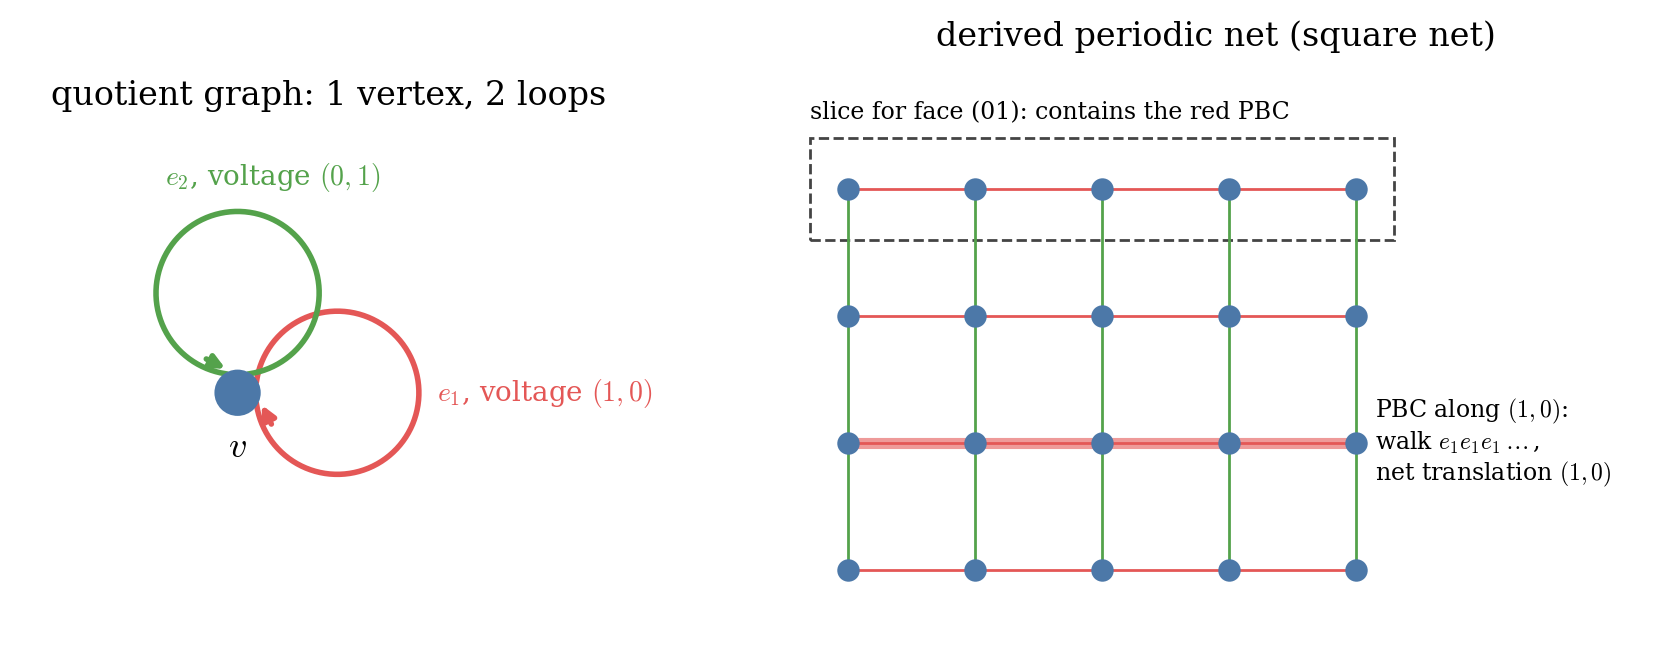
\includegraphics[width=.9\linewidth]{quotient.png}
\caption{Left: a quotient graph with one vertex and two loop edges, carrying voltages $(1,0)$ and $(0,1)$. Right: the periodic net it describes (a square net). Walking $e_1e_1e_1\dots$ traces a straight chain with net translation $(1,0)$, which is a periodic bond chain.}
\label{fig:quot}
\end{figure}

\paragraph{Net voltage of a cycle.} For a closed walk $W$ in the quotient graph, its \textbf{net voltage} $\nu(W)$ is the sum of the voltages along it (counting an edge traversed backwards with a minus sign). In the earlier work we defined the \textbf{periodicity rank} $\varrho$ as the rank of the set of all net voltages. It is 3 for a 3D framework, 2 for layers, 1 for chains and 0 for isolated clusters, and we used it in the linker-deletion ladder 3D$\to$2D$\to$1D$\to$0D for MOF-5.

\section{Periodic bond chains as cycles: our proposed bridge}

Here is the connection to Hartman--Perdok theory. It is the most original part of our plan, so we state it carefully as a proposal to be tested.

\begin{proposition}[PBCs are cycles with non-zero net voltage]\label{prop:pbc}
A closed walk $W$ of strong-bond edges in the quotient graph with $\nu(W)=\vect{\tau}\ne\vect{0}$ lifts to an infinite chain in the crystal that repeats with translation $\vect{\tau}$. That chain is a periodic bond chain. It is parallel to the face $(hkl)$ if and only if
\begin{equation}
h\tau_1+k\tau_2+l\tau_3=0.
\end{equation}
\end{proposition}
\begin{proof}[Proof sketch]
Lifting each edge adds its voltage to the cell index, so after one traversal of $W$ the walk returns to the same node, shifted by $\vect{\tau}$, and repeating it gives an infinite periodic chain. A lattice vector $\vect{\tau}$ lies in the plane $(hkl)$ exactly when it is perpendicular to $\vect{g}_{hkl}$, which in fractional coordinates is $\vect{h}\cdot\vect{\tau}=0$.
\end{proof}

\begin{keyidea}[title=Our proposal]
For each face $(hkl)$, take the strong-bond edges whose atoms lie in a slice of thickness $d_{hkl}$. Compute the rank of the net voltages of their cycles. This is the periodicity rank of the slice subgraph. Then:
\[
\text{rank }2\Rightarrow\text{F face},\qquad\text{rank }1\Rightarrow\text{S face},\qquad\text{rank }0\Rightarrow\text{K face}.
\]
This reuses the periodicity rank from our earlier work, applied to a slab instead of to the whole crystal.
\end{keyidea}

\begin{careful}
\begin{itemize}
\item The condition $\vect{h}\cdot\vect{\tau}=0$ alone is not enough. In the simple cubic crystal of \autoref{fig:fsk}, a zigzag chain along $[1\bar10]$ also satisfies it for $(110)$, yet the standard treatment classifies $(110)$ as an S face. What decides this is the slice condition (which bonds lie inside the slab of thickness $d_{110}$), which uses atom positions. We must implement that condition carefully and test it on this textbook case first.
\item We must choose which bonds count as ``strong''. For MOFs the natural choice is the metal--linker coordination bonds. This is a modelling decision and must be stated.
\item MOF faces can be cut in several ways (different terminations). Each must be checked.
\end{itemize}
\end{careful}

\section{Counting connections: a graph rule for growth rates}\label{sec:attach}

Here is a second way to get growth rates from the graph, simpler than bond chains: count how many links a new node forms when it lands on a face. Chen et al.\ used exactly this argument to explain the shapes of real UiO-67 crystals (\autoref{sec:chen} describes their experiments). We state it as a graph quantity and compute it ourselves.

\begin{definition}[Attachment number]
Let $N$ be the periodic net of nodes and linkers. Cut it along a plane parallel to the face $(hkl)$, keeping the nodes on one side as ``the crystal''. For a node position in the next layer, count its edges to nodes already in the crystal. The largest such count over the next-layer positions is the \textbf{attachment number} $c_{hkl}$.
\end{definition}

A node with more links to the crystal is held more firmly, so it attaches and stays more easily, and the face grows faster:
\begin{equation}\label{eq:attach}
R_{hkl}\ \text{increases with}\ c_{hkl}.
\end{equation}
This is the graph version of the attachment-energy rule of \autoref{sec:wulff}, where each link counts as one unit of bond energy.

\begin{figure}[H]\centering
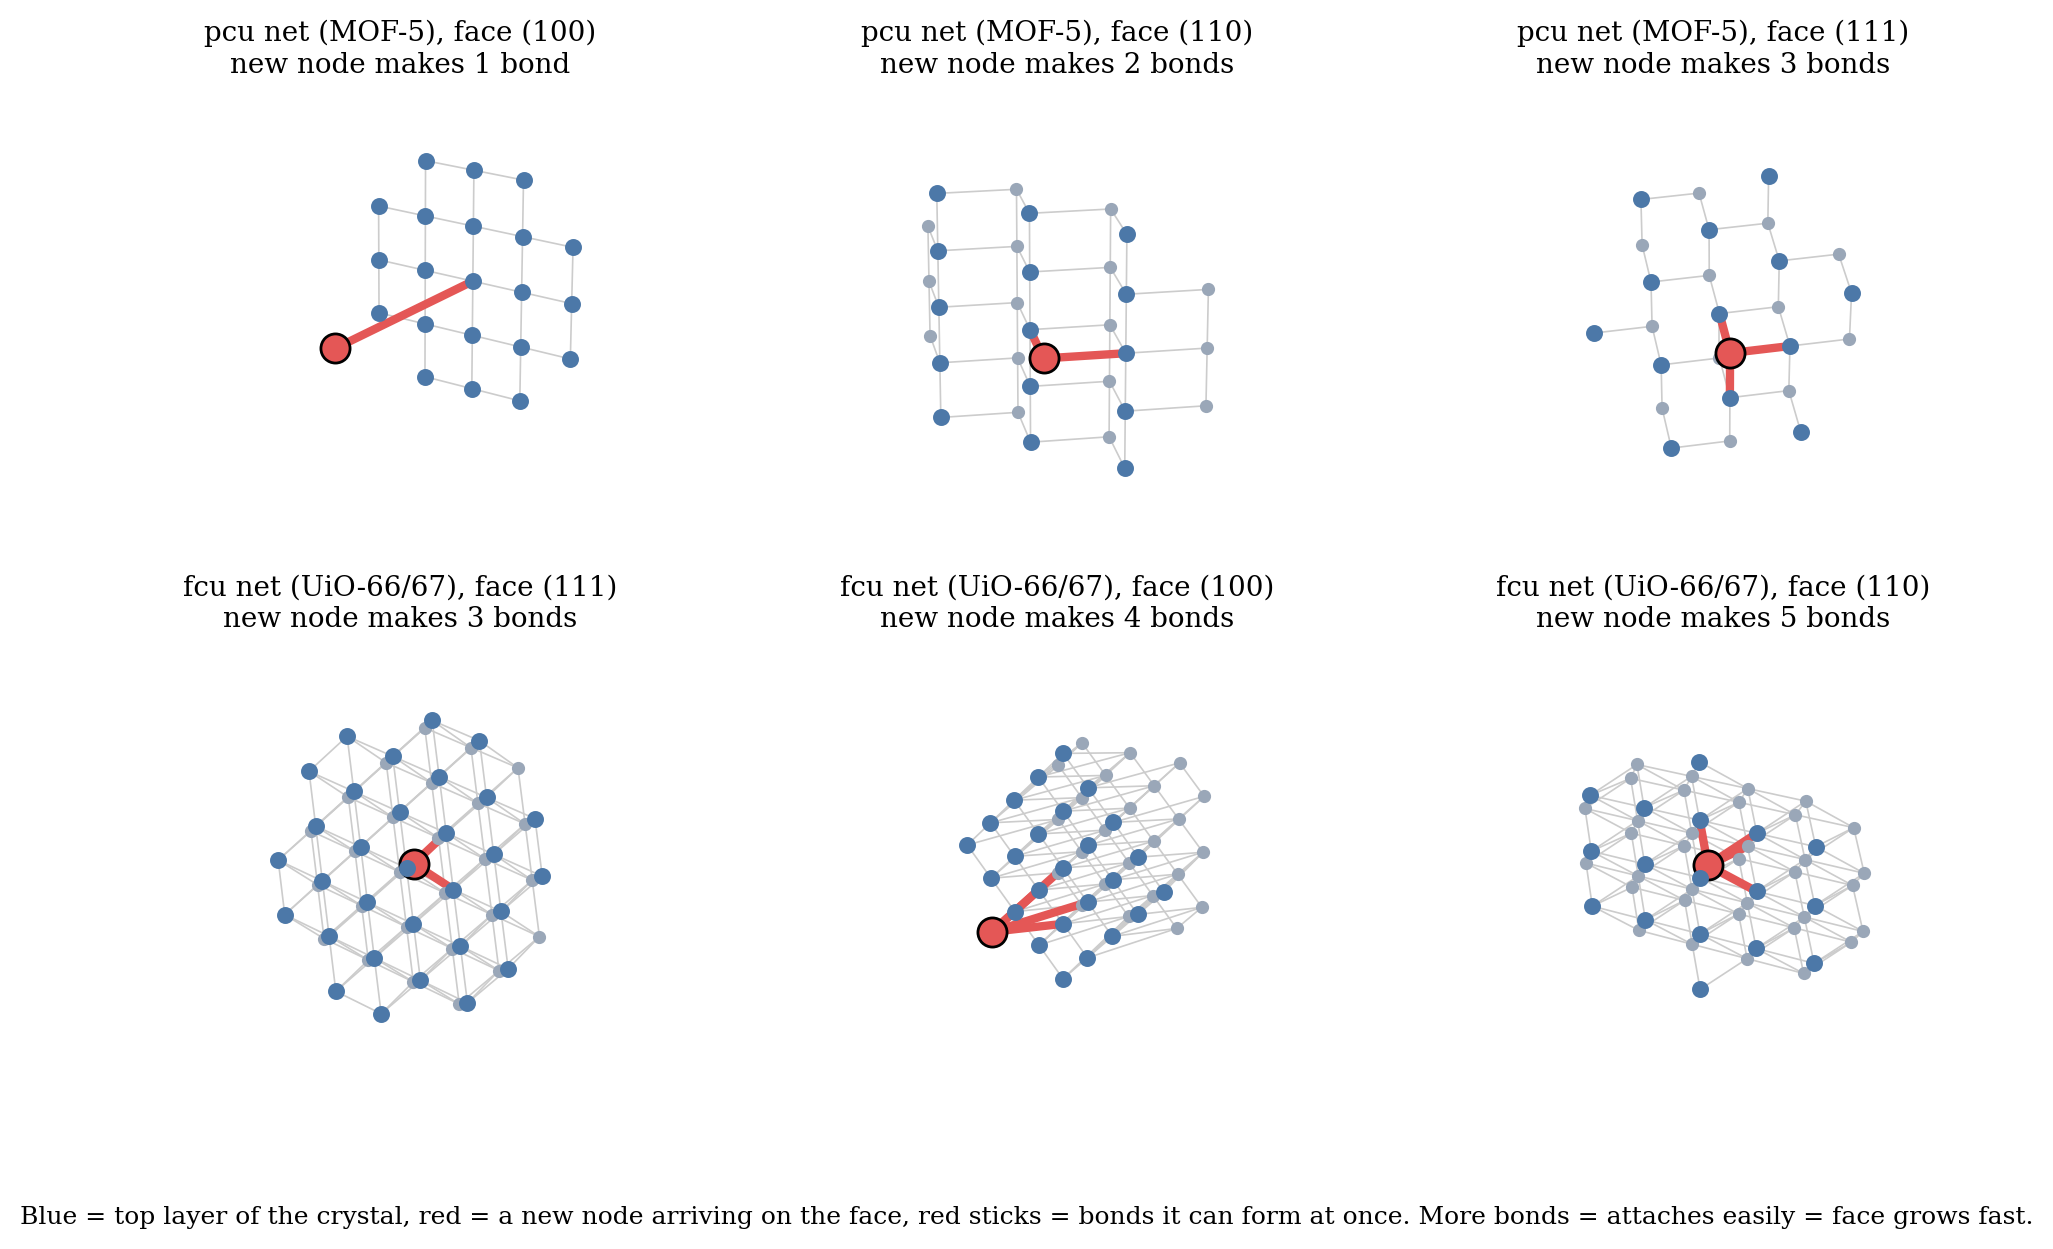
\includegraphics[width=\linewidth]{attach.png}
\caption{Attachment numbers computed by us on the node nets. Top: pcu (MOF-5) gives 1, 2 and 3 for (100), (110) and (111). Bottom: fcu (UiO-66/67) gives 3, 4 and 5 for (111), (100) and (110), reproducing the numbers stated by Chen et al.}
\label{fig:attach}
\end{figure}

\begin{table}[H]\centering\small
\begin{tabular}{lcccl}
\toprule
Net (MOF) & $c_{100}$ & $c_{110}$ & $c_{111}$ & Predicted shape (slowest faces)\\
\midrule
pcu (MOF-5) & 1 & 2 & 3 & \textbf{cube} $\{100\}$ \\
fcu (UiO-66/67) & 4 & 5 & 3 & \textbf{octahedron} $\{111\}$, via cuboctahedron \\
sod (ZIF-8) & 1--2 & 1--2 & 1 & not resolved by this simple count \\
\bottomrule
\end{tabular}
\caption{Attachment numbers from our code. For sod the count depends on where the plane cuts the net, so a single number per face is not enough.}
\label{tab:attach}
\end{table}

\begin{keyidea}
For MOF-5 this simple graph rule predicts \textbf{cubes}, the shape usually reported in experiments, where BFDH predicted an octahedron (\autoref{sec:bfdh}). The difference is that BFDH looks at the atoms' lattice, while the attachment number looks at the \emph{connectivity of the framework}. That is strong evidence that our graph approach adds something real.
\end{keyidea}

\begin{careful}
\begin{itemize}
\item For MOF-5 we used the net of Zn$_4$O nodes, which is primitive cubic with spacing $a/2$. The face directions are the same as in the Fm$\bar3$m cell.
\item The count treats all links as equal and ignores solvent, modulators and how strongly each link binds. It is a first-order rule.
\item For sod (ZIF-8) the single-node count does not separate the faces, even though experiments and BFDH both give rhombic dodecahedra. A better rule, such as counting links per unit area for a whole new layer, or the Hartman--Perdok slice analysis of \autoref{prop:pbc}, is needed. This is a concrete task for Phase 3.
\end{itemize}
\end{careful}

%=====================================================================
\part{What the reference papers contribute}
%=====================================================================
\section{Wu \& Jiang (Chem.\ Sci.\ 2024): node shapes and chemistry tools}

\textbf{X.~Wu and J.~Jiang, ``Precision-engineered metal--organic frameworks: fine-tuning reverse topological structure prediction and design'', Chem.\ Sci.\ 15, 16467 (2024).} Our faculty recommended this paper. We read the methods and most of the results.

\paragraph{What they did.} They generate new MOFs by the \emph{reverse topological approach}: start from a target net, then fill its vertices and edges with building units. Their improvement, called precision engineering (PE), is a strict geometry check before assembly.
\begin{itemize}
\item \textbf{Geometric signatures.} Every building unit is classified into one of 13 shape prototypes by its connection points: linear (L2), triangle (T3), square (S4), tetrahedron (T4), hexagon (H6), octahedron (O6), trigonal prism (T6), cube (C8), cuboctahedron (C12), icosahedron (I12), hexagonal prism (H12), truncated tetrahedron (T12) and truncated octahedron (T24). The classification uses the number of connection points, a planarity test, and the smallest root-mean-square deviation (RMSD) from the ideal prototypes (\autoref{fig:proto}).
\item \textbf{Topological constraints.} A reference table says which pairs of signatures fit which net. For example, the Cu paddlewheel (S4) with BTC (T3) gives the tbo net, which is HKUST-1.
\item \textbf{Assembly and relaxation.} They built 200,875 structures with the PORMAKE code (RMSD cut-off 0.3\,\AA) and kept 94,823 after relaxing them with the UFF force field and machine-learned PACMOF charges.
\item \textbf{Screening.} They computed pore descriptors with Zeo++ and simulated CO$_2$/N$_2$ adsorption with RASPA. 1,207 of their MOFs beat zeolite 13X on their trade-off score. The best reached 8.28\,mol\,kg$^{-1}$ CO$_2$ uptake with CO$_2$/N$_2$ selectivity 346 at 1\,bar.
\end{itemize}

\begin{figure}[H]\centering
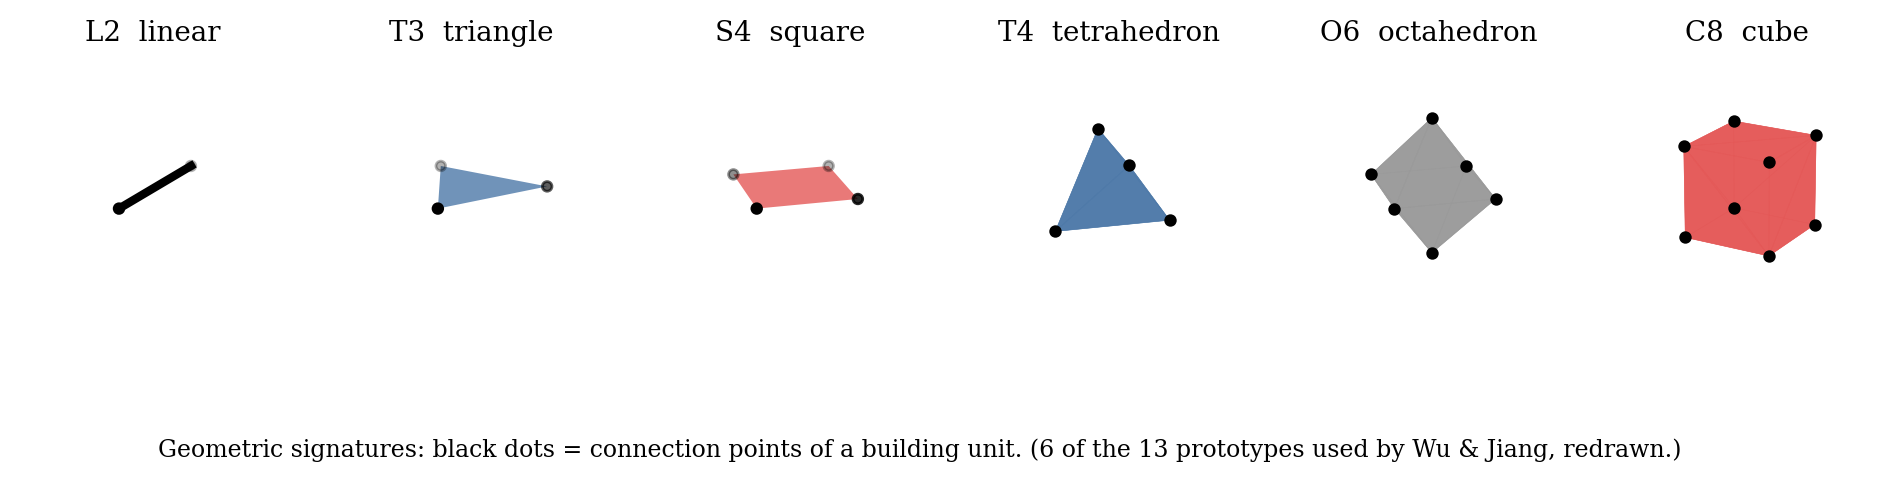
\includegraphics[width=\linewidth]{prototypes.png}
\caption{Six of the 13 geometric signatures used by Wu \& Jiang, redrawn by us. Black dots are connection points.}
\label{fig:proto}
\end{figure}

\begin{forus}
\begin{itemize}
\item The geometric signatures give a precise vocabulary for \emph{node} shape (level (a) in \autoref{fig:levels}). We can label our nodes the same way.
\item Their UFF relaxation workflow is the template for our surface-energy calculations in the Wulff step.
\item Zeo++ and RASPA link morphology back to the project's original goal, adsorption.
\item Limitation: the paper does not deal with crystal morphology at all. It concerns structure, not particle shape.
\end{itemize}
\end{forus}

\section{Chen et al.\ (Matter 2020): real MOF crystals change shape}\label{sec:chen}

\textbf{P.~Chen, Z.~Tang, Z.~Zeng, \dots, D.~Zhou, C.~Wang, W.~Lin, ``Machine-learning-guided morphology engineering of nanoscale metal-organic frameworks'', Matter 2, 1651--1666 (2020), doi:10.1016/j.matt.2020.04.021.} Our teammate found this paper, and we have read the full text. It is the closest experimental paper to our question.

\subsection{The system}
They made nanoscale MOFs from HfCl$_4$ (or ZrCl$_4$) and biphenyl-4,4$'$-dicarboxylic acid (H$_2$BPDC) in DMF solvent, with water and formic acid added. Three crystal phases form:
\begin{itemize}
\item \textbf{UiO-67}: the same fcu net as UiO-66, with the longer BPDC linker. Each Hf$_6$ cluster is 12-connected. It is F-centred cubic, so everything in Parts II--IV applies.
\item \textbf{hcp-UiO-67}: a \emph{different} structure built from Hf$_{12}$ clusters (18-connected) in hexagonal close packing. It grows as hexagonal nanoplates.
\item \textbf{hxl-UiO-67}: closely related to hcp-UiO-67 but disordered perpendicular to the plates. It grows as thin plates, down to single layers.
\end{itemize}
A Hf-formate phase and undissolved H$_2$BPDC also appear under some conditions.

\begin{careful}
The hexagonal plates are a different crystal structure, with a different unit cell, not a different shape of the UiO-67 unit cell. For our question (``many shapes from \emph{one} unit cell''), the relevant UiO-67 shapes are the sphere-like ``ball'', the cuboctahedron, and the octahedron. The concave and hollow octahedra come from dissolving and regrowing an existing crystal.
\end{careful}

\subsection{Machine learning of the phase diagram}
\begin{itemize}
\item They ran 287 syntheses, spreading the conditions evenly with a ``uniform design'' algorithm, for 24\,h each, varying the temperature and the amounts of HfCl$_4$, H$_2$BPDC, DMF, water and formic acid. Each product's phase was identified by powder X-ray diffraction.
\item A decision tree (CART, with Gini impurity) found that \textbf{temperature, water concentration and formic acid concentration} matter most.
\item With temperature fixed at 150\,$^\circ$C, a random forest of 1,000 ``multivariate decision trees'' (trees whose splits are tilted lines in the water/formic-acid plane) drew the phase diagram, with about 80\% test accuracy. Overlapping regions are mixed phases.
\end{itemize}

\subsection{Clusters in solution and the growth mechanism}
\begin{itemize}
\item Liquid-cell TEM and mass spectrometry detected both Hf$_6$ clusters (about 1.4\,nm) and Hf$_{12}$ clusters (about 2.2\,nm $\times$ 1.4\,nm) in solution \emph{before} any crystals formed. The [Hf$_{12}$]/[Hf$_6$] ratio follows the phase domains: where Hf$_{12}$ dominates, the hcp and hxl phases form.
\item Their proposed mechanism: the clusters form first, capped by formate, and the crystal grows when BPDC linkers replace the formate caps (ligand exchange). Linking two clusters with one BPDC releases two formates, which gains entropy. Two Hf$_{12}$ clusters can be doubly linked sideways, which favours sideways growth and explains why the Hf$_{12}$ phases grow as plates.
\end{itemize}

\subsection{Measuring plate thickness with a neural network}
They collected 1,510 SEM images from 69 conditions. A Mask R-CNN network, fine-tuned on 228 hand-labelled images, cut out plates standing on edge, and Gaussian fits of the image brightness gave the thickness. On a 31-image test set it reached 0.81 average precision, with 10\% error in length and 14\% in thickness. Thickness ranged from about 111\,nm down to a 1.3\,nm monolayer (measured by AFM), with a hexagonal lattice of clusters 1.94\,nm apart. Thickness grew with lateral size, so the ratio of sideways to vertical growth rate stays in a narrow range. A random forest ranked the H$_2$BPDC concentration as the most important variable for thickness.

\subsection{The key result for us: growth rate from counting connections}
The paper explains the UiO-67 shapes with a simple counting argument:
\begin{quote}
A cluster added to the (110) face of UiO-67 can form \textbf{five} connections with existing clusters. On the (100) face it forms \textbf{four}, and on the (111) face \textbf{three}. This gives a growth-rate order (110) $>$ (100) $>$ (111). The faces that remain are the slowest-growing ones, so the shape evolves from a \textbf{ball} to a \textbf{cuboctahedron} (with (100) and (111) faces) to an \textbf{octahedron} (with only (111) faces).
\end{quote}
Their synthesis recipes confirm the time order. The cuboctahedra were made with the reaction stopped at 1.5\,h, and the octahedra after one day, under nearly the same conditions.

\begin{forus}
This is exactly the morph path of \autoref{fig:morph}, travelled in time, and exactly the mechanism of \autoref{fig:growth}: the fast $\{100\}$ faces shrink until only $\{111\}$ remains. Their argument is purely graph-theoretic, since it counts edges of the fcu net. We turn it into a general tool in \autoref{sec:attach}.
\end{forus}

\subsection{Designing complex shapes by epitaxy}
\begin{itemize}
\item \textbf{Hollow octahedra}: UiO-67 octahedra moved into the conditions that grow hcp-UiO-67. Hf$_{12}$ clusters add epitaxially on the (111) faces and lock them, while the inside of the octahedron dissolves. The hollow octahedron then turns into triangular, truncated-triangular and finally hexagonal plates.
\item \textbf{Concave octahedra}: UiO-67 octahedra moved into the conditions that grow Hf-formate. The formate phase grows on the (110) edges and locks them, while the faces dissolve.
\item The same strategy worked for UiO-68 with a nitro-terphenyl linker, giving octahedra, nanoplates and hollow octahedra ``without extensive trials''. Thermogravimetric analysis showed many missing-linker defects in all samples.
\end{itemize}

\subsection{Shape changes function}
With a bipyridine linker (BPYDC) and Co added, the MOFs catalysed olefin hydrogenation. For styrene the turnover numbers were: hollow octahedron 386, octahedron 210, nanoplate 143, 2D nanosheet 111. For the larger trans-$\beta$-methylstyrene: 318, 117, 82 and 84. The concave octahedra could not be loaded with Co, probably because Hf-formate blocks the pores. So morphology changes performance by up to about four times, which links morphology back to our project's original goal.

\begin{forus}
\begin{itemize}
\item This is the chemical proof the panel mentioned: one MOF chemistry, many morphologies, controlled by synthesis conditions.
\item For a single unit cell (UiO-67) they observe the ball $\to$ cuboctahedron $\to$ octahedron sequence. Our mathematics reproduces it (\autoref{fig:morph}), and so does their connection counting, which we reproduce in \autoref{sec:attach}.
\item Plates in their work come from a different phase, so our stretched shapes (\autoref{fig:rod}) are not a model of their plates. They remain a model for anisotropic growth of a single phase.
\item Concave and hollow shapes are not convex and come from dissolution, so they are outside our polytope model.
\item Their code is public (github.com/Wang-Group/CPC-code and github.com/zmzeng/Mask\_RCNN).
\end{itemize}
\end{forus}

\section{The earlier references and our own earlier work}

\paragraph{Chen et al., Science Advances 12, eaee8016 (2026)} computes topological features separately for each chemical element and combines them in a transformer model. Its message for us is that adsorption depends mostly on pore topology, while some properties need element-aware features. \textbf{Anselmi et al., J.\ Mater.\ Chem.\ A 14, 7628 (2026)} screens MOF photocatalysts with graph-based machine learning. Neither is about crystal morphology, so both are background for this phase.

\paragraph{Our earlier work} gave three things we keep: the periodic quotient graph, the periodicity rank, and shape descriptors. The multifractal ($\Delta\alpha$) route was shown to depend on system size and is kept only as a documented negative result.

%=====================================================================
\part{Putting it together}
%=====================================================================
\section{The pipeline}

\begin{figure}[H]\centering
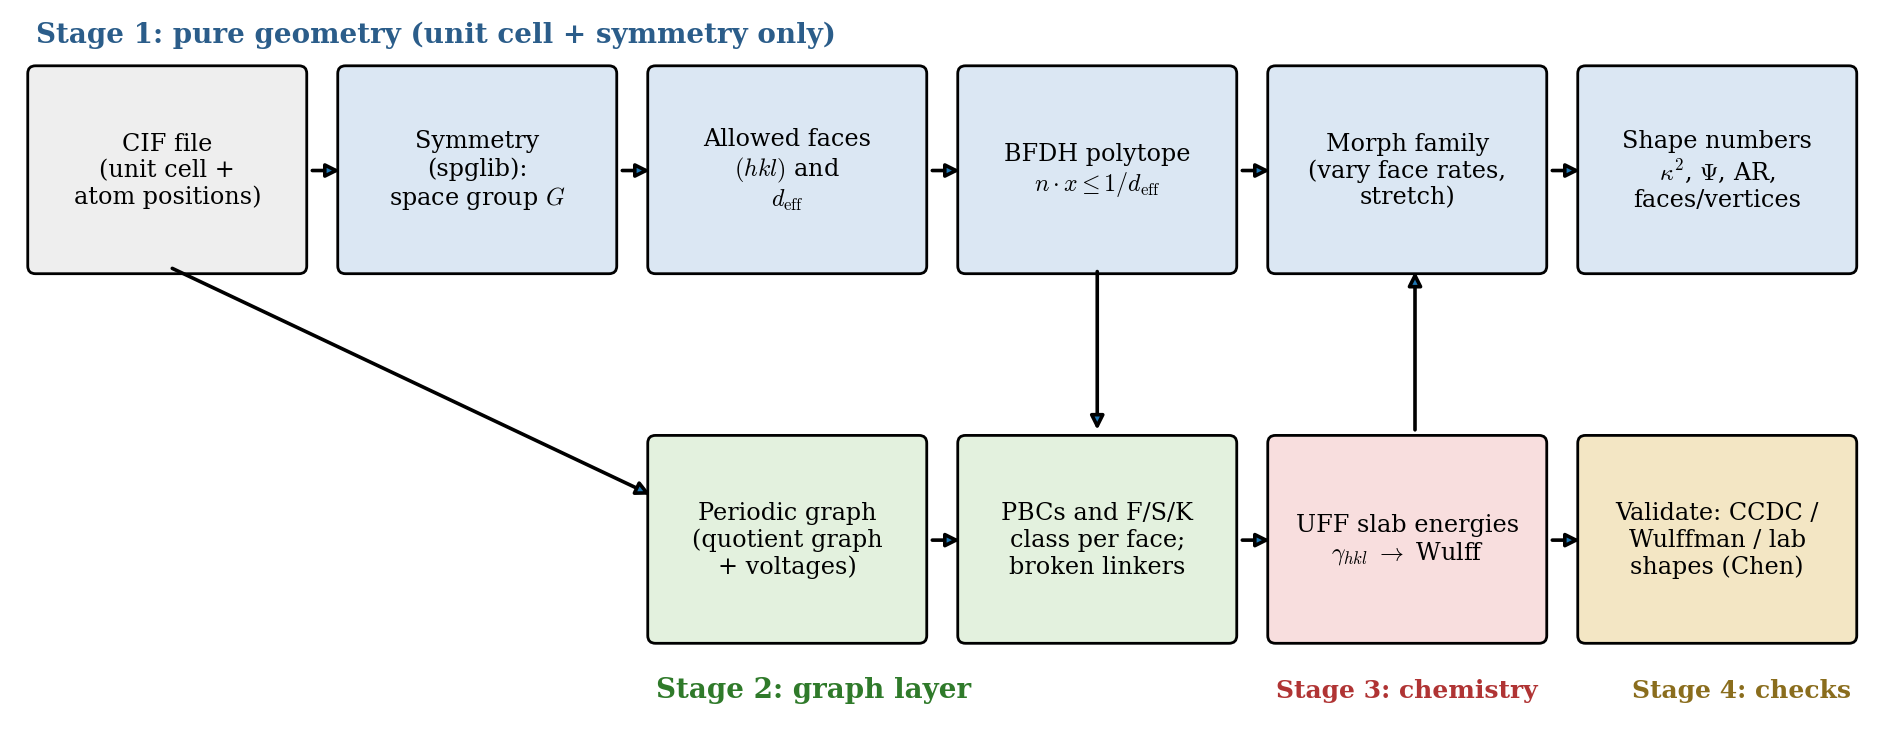
\includegraphics[width=\linewidth]{pipeline.png}
\caption{The full pipeline. Stage 1 (blue) answers the panel's question using only the unit cell. Stage 2 (green) adds our graph-based face classification. Stage 3 (red) adds chemistry through surface energies. Stage 4 checks everything against trusted tools and experiments.}
\label{fig:pipe}
\end{figure}

\section{Detailed work plan}

\subsection*{Phase 0: Preparation}
\begin{itemize}
\item Read this primer, then the Hartman--Perdok revisited paper (Grimbergen et al.\ 1998) and the full Chen et al.\ paper.
\item Collect specific literature references for the experimental shapes of MOF-5, HKUST-1, UiO-66 and ZIF-8.
\item Run a proper literature search for MOF morphology predicted by BFDH, attachment energy or Wulff, so we know what has already been done before claiming novelty.
\item \emph{Output:} one-page problem statement and a table of related work.
\end{itemize}

\subsection*{Phase 1: Geometry from the unit cell (Stage 1)}
\begin{enumerate}
\item Read each CIF and convert it to the conventional cell.
\item Detect the space group with spglib, with and without hydrogens, at several tolerances (\autoref{sec:ourmofs}).
\item For all $(hkl)$ up to index 6, apply \autoref{prop:abs} with the full list of symmetry operations to find allowed faces and $d_{\text{eff}}$.
\item Build the BFDH polytope \eqref{eq:polytope} with \eqref{eq:bfdh}.
\item Generate the morph family by varying $t$ and $\lambda$ (\autoref{sec:morph}).
\item Compute sphericity, face and vertex counts, aspect ratio and $\kappa^2$ (\autoref{sec:measure}). Add a face-normal order parameter to separate cubic-symmetric shapes.
\item Render every shape.
\end{enumerate}
\emph{Output:} code, results table and images. This phase alone answers the panel's question.

\subsection*{Phase 2: Mathematical statements}
Write Propositions~\ref{prop:abs}--\ref{prop:pbc} cleanly, with full proofs where we can and citations where the result is classical (Wulff).

\subsection*{Phase 3: Graph layer (Stage 2)}
\begin{enumerate}
\item Rebuild the quotient graph of each MOF with metal-cluster nodes and linker edges.
\item Mark the strong bonds (metal--linker coordination bonds) and state this choice.
\item For each face, extract the slice subgraph and compute its periodicity rank, giving F, S or K (\autoref{prop:pbc}).
\item Carve a supercell along the BFDH planes and count broken linkers and under-coordinated nodes on each face.
\item Compute attachment numbers $c_{hkl}$ (\autoref{sec:attach}) for all four nets, including the two node types of tbo (HKUST-1), and fix the sod case with a per-layer or per-area count.
\item Check whether the F faces and low-$c_{hkl}$ faces from the graph agree with each other, with BFDH, and with experiment.
\end{enumerate}

\subsection*{Phase 4: Chemistry layer (Stage 3)}
\begin{enumerate}
\item Build slab models for the leading faces, with every reasonable termination.
\item Compute surface energies $\gamma_{hkl}$ with UFF, following the Wu \& Jiang workflow.
\item Build the Wulff shape \eqref{eq:wulff} and compare it with BFDH.
\item Test the MOF-5 case: does the chemistry layer turn the BFDH octahedron into the observed cube?
\end{enumerate}

\subsection*{Phase 5: Validation (Stage 4)}
\begin{itemize}
\item Compare our BFDH shapes with the CCDC particle-shape tool or Materials Studio, and our Wulff shapes with NIST Wulffman.
\item Compare with experimental shapes, including Chen et al.
\item Report agreements and disagreements honestly.
\end{itemize}

\subsection*{Phase 6: Write-up}
Introduction, background (this primer, shortened), theory, methods, results for four MOFs, validation, the multifractal negative result as an appendix, and limits.

\section{What we can and cannot claim}
\begin{itemize}
\item \textbf{We can claim:} from the unit cell and symmetry alone, a family of morphologies follows mathematically. We can show which shapes appear for which growth-rate ratios, and measure them with numbers.
\item \textbf{Already shown in this primer:} the attachment-number rule on the node net reproduces Chen et al.'s UiO-67 counts and predicts the cube shape of MOF-5 where BFDH fails.
\item \textbf{We can claim (after Phases 3--4):} a graph-based classification of faces and a chemistry-based estimate of which shape is favoured.
\item \textbf{We cannot claim:} that a given lab synthesis will produce a given shape. Real shapes also depend on solvent, temperature, concentration and modulators (Chen et al.). Our shapes are the morphologies the structure \emph{allows}.
\item \textbf{We cannot claim novelty} until the Phase~0 literature search is done. The individual methods are old and well established. What may be new is joining them to MOF periodic graphs.
\end{itemize}

%=====================================================================
\appendix
\section{Glossary}
\begin{description}[style=nextline,leftmargin=1.2em]
\item[Attachment energy] Energy released when a new slice attaches to a face. Used as a growth-rate estimate.
\item[BFDH] Rule that growth rate $\propto 1/d_{\text{eff}}$. Needs only the unit cell and space group.
\item[Centring (F, I)] Extra lattice points at face centres (F) or the body centre (I) of the conventional cell.
\item[CIF] Crystallographic Information File: unit cell, symmetry and atom positions.
\item[Conventional / primitive cell] Symmetry-aligned cell versus smallest possible cell.
\item[$d_{hkl}$, $d_{\text{eff}}$] Spacing between $(hkl)$ planes; spacing after systematic absences are applied.
\item[F / S / K face] Flat, stepped and kinked faces, with PBCs in two, one or no directions.
\item[Habit / morphology] Outer shape of the crystal particle.
\item[Miller indices $(hkl)$] Integer names for planes; $\{hkl\}$ is the symmetry-equivalent family.
\item[Net / topology] Connection pattern of nodes and linkers (pcu, tbo, fcu, sod).
\item[PBC] Periodic bond chain: an unbroken chain of strong bonds repeating with a lattice translation.
\item[Periodicity rank] Rank of the net voltages of a periodic graph: 3, 2, 1 or 0.
\item[Quotient graph, voltage] One-cell graph whose edges carry the lattice shift they cross.
\item[Space group] Complete set of symmetry operations of a crystal (230 types).
\item[Sphericity $\Psi$] $\pi^{1/3}(6V)^{2/3}/A$, which is 1 for a sphere.
\item[Systematic absence] A plane family forbidden by symmetry (\autoref{prop:abs}).
\item[UFF] Universal Force Field, a simple force field for any element.
\item[Wulff shape] Equilibrium crystal shape from surface energies.
\end{description}

\section{Self-test questions}
Answer these before starting Phase 1. Answers are below.
\begin{enumerate}
\item Why do our HKUST-1 and UiO-66 CIFs show $60^\circ$ angles if the crystals are cubic?
\item For an F-centred cubic crystal, why does the cube face have $d_{\text{eff}}=a/2$ and not $a$?
\item Which faces does BFDH predict for ZIF-8, and why?
\item In \autoref{fig:growth}, why do the fast faces disappear?
\item For $\{100\}$ at distance 1, what value of $t$ gives a cuboctahedron?
\item Why is $\kappa^2=0$ for both a cube and an octahedron?
\item What is the difference between an F face and a K face?
\item In graph terms, when is a cycle in the quotient graph a PBC parallel to $(hkl)$?
\item Which of Chen et al.'s shapes can our polytope model not produce, and why?
\item Why does the attachment-number rule predict cubes for MOF-5 but octahedra for UiO-66?
\end{enumerate}
\paragraph{Answers.}
(1) The file stores the primitive cell of an F-centred lattice; the conventional cell is cubic with $a=\sqrt2\,a_{\text{prim}}$.
(2) The face-centring translation puts identical planes halfway between the $(100)$ planes, so $(100)$ is absent and the first allowed reflection is $(200)$.
(3) $\{110\}$, a rhombic dodecahedron, because I-centring forbids $(100)$ and $(111)$ and $\{110\}$ has the largest remaining spacing.
(4) Each face's distance grows in proportion to its rate, so fast faces are overtaken by their slow neighbours.
(5) $t=2/\sqrt3\approx1.155$.
(6) Both have cubic symmetry, which forces the gyration tensor to be a multiple of the identity (\autoref{prop:k2}).
(7) An F face's slice contains PBCs in two independent directions, a K face's slice contains none.
(8) When its net voltage $\vect{\tau}\neq\vect0$ satisfies $h\tau_1+k\tau_2+l\tau_3=0$ and the chain fits in the $d_{hkl}$ slice.
(9) Concave and hollow octahedra, because the model only produces convex shapes (and their hexagonal plates are a different phase).
(10) In pcu a new node on (100) makes only 1 link, so $\{100\}$ grows slowest and survives; in fcu the (111) face gives the fewest links (3), so $\{111\}$ survives.

\section{Reading list and references}
Items marked $\dagger$ we have seen only as a title or abstract. Items marked $\ddagger$ are cited from general knowledge; check the exact details before citing them in the final paper.
\begin{enumerate}[label={[\arabic*]}]
\item X.~Wu, J.~Jiang, Chem.\ Sci.\ 15, 16467 (2024). Read in full for methods.
\item P.~Chen et al., Matter 2, 1651 (2020), doi:10.1016/j.matt.2020.04.021. Read in full.
\item R.~F.~P.~Grimbergen, H.~Meekes, P.~Bennema, C.~S.~Strom, L.~J.~P.~Vogels, ``On the prediction of crystal morphology. I. The Hartman--Perdok theory revisited'', Acta Cryst.\ A 54, 491 (1998).$\dagger$
\item P.~Hartman, ``Crystal faces: structure and growth'', Netherlands J.\ Geosciences 61, 313 (1982).$\dagger$
\item S.~Miracle-Sol\'e, ``Wulff shape of equilibrium crystals'', arXiv:1307.5180 (2013).$\dagger$
\item P.~Hartman, W.~G.~Perdok, Acta Cryst.\ 8 (1955): the original PBC papers.$\ddagger$
\item P.~Hartman, P.~Bennema, J.\ Cryst.\ Growth 49, 145 (1980): attachment energy and growth rate.$\ddagger$
\item J.~D.~H.~Donnay, D.~Harker, Am.\ Mineral.\ 22, 446 (1937): the BFDH law with screw and glide corrections.$\ddagger$
\item G.~Wulff, Z.\ Kristallogr.\ 34, 449 (1901); J.~E.~Taylor, Bull.\ AMS 84, 568 (1978): the Wulff theorem.$\ddagger$
\item CCDC, ``Particle shape calculation using CSD-Particle'' (tutorial); NIST Wulffman (software).
\item D.~Chen et al., Sci.\ Adv.\ 12, eaee8016 (2026); M.~Anselmi et al., J.\ Mater.\ Chem.\ A 14, 7628 (2026).
\item A.~Togo et al., spglib, a library for crystal symmetry search (software).
\end{enumerate}

\end{document}
